\chapter{Introduction}
\label{ch:Intro}


%%%%%%%%%%%%%%%%%%%%%%%%%%%%%%%%%%%%%%%%%%%%%%%%%%

Our growing knowledge of genetic associations with susceptibility to psoriasis and psoriatic arthritis (PsA) has not yet been matched by understanding the functional basis of these disease-specific associations and the translation to patients' benefit. To address this challenge, it is important to understand the regulatory genomic landscape within which disease-associated genetic variants may act. This thesis describes functional genomic approaches to establish genome-wide epigenetic and gene expression profiles for disease relevant tissues and blood-isolated immune cells in psoriasis and PsA, and explore their potential significance for disease pathogenesis and genetic variation. In this chapter, I begin by reviewing current knowledge of the pathophysiology of psoriasis and psoriatic arthritis, the role of genetic variation, and the challenge of functionally characterising genome-wide association studies (GWAS) in complex traits, including the different functional genomics approaches that can be applied.

\section{Psoriasis and psoriatic arthritis}
%
Psoriasis and PsA have been described are common complex disease entities that nonetheless share certain clinical features and genetic architecture. Psoriasis is a chronic inflammatory skin disease characterised by episodes of relapse and remittance, most commonly manifesting as well-demarcated erythematous plaques with silver scale and associated with increased risk of joint, eye and systemic disorders \parencite{Nestle2009}. On the other hand, PsA is a seronegative chronic inflammatory disease within the spondyloarthritis (SpA) family that usually develops after psoriasis skin manifestations \parencite{Moll1973, Coates2016, Villanova2013}. Both conditions present similarities and differences at the pathophysiological and genetic level.

%(Variants in RUNX3 contribute to susceptibility to PsA, exhibiting further common ground with ankylosing spondylitis, PsA Immunochip)

\subsection{Epidemiology and global impact}
%
Psoriasis represents a serious global health problem that currently affects about 100 million people worldwide, including both children and adults with  no sex bias \parencite{Organization2016}. Although the mean age of onset is 33 years, a bimodal distribution with psoriasis patients being classified as early-onset/ type I (with peaks between 16 and 22 years) or late-onset / type II (between 50-60 years) has also been described \parencite{Henseler1985, Perera2012}. This classification based on the age of onset also correlates with distinctive clinical features including severity, relapse frequency and family history. 

The risk of developing psoriasis shows ethnic differences with a lower prevalence among adult African, African American and Asian populations (between 0.4 and 0.7\%) compared to American and Canadian (4.6 and 4.7 \%, respectively) \parencite{Jacobson2011}. In the UK the prevalence of psoriasis ranges between 2 and 3\%, affecting approximately 1.8 million people \parencite{Perera2012}. \ToDo{For PsA, incidence in the general population varies between 0.04 and 1.2\%, with peak age of onset between the 35 and 45 years of age. The estimation of psoriasis patients with concominant PsA ranges from 10 to 30\%, with arthritis onset occurring approximately ten years after the onset of the skin disease \parencite{Greb2016}. This clearly evidences the strong association between both diseases \parencite{Gelfand2005,Reich2015,Perera2012}.}


Several severe comorbidities are associated with psoriasis and PsA, with comparatively greater prevalence in PsA. For example, intraocular inflammation (uveitis) affects 8\% of PsA patients compared to only 2\% of psoriasis patients \parencite{Husted2011, Oliveira2015}. Other comorbidities include inflammatory bowel disease (IBD), cardiovascular disease (CVD), type 2 diabetes (T2D) and metabolic syndrome \parencite{Gelfand2006,Shapiro2007,Cohen2008}. Psoriasis and PsA have also been associated with an increased prevalence of depression and suicidal ideation, and they represent a significant burden for the economy due to treatment costs and associated morbidity \parencite{Sampogna2012}.  In fact, treatment and management-associated costs per psoriasis patient in UK during 2015 accounted for \textsterling4,000 to \textsterling14,000, before and after requirements of biological therapy, respectively, and were larger in PsA \parencite{Burgos-Pol2016}.




\subsection{Psoriasis and inflammatory dermatoses}
%

The skin is the biggest organ in the human body and constitutes an effective barrier between the environment and the internal organs. The most external layer, the epidermis, plays an important role in innate and adaptive immunity and its alterations can lead to development of inflammatory skin conditions, such as psoriasis or atopic dermatitis \parencite{Johnson-Huang2009, Proksch2008}. Lesions in psoriasis are very heterogeneous in type (pustular and non- pustular), location and severity, which complicates its clinical classification \parencite{Perera2012}. As a result, several phenotypes  including chronic plaque psoriasis (psoriasis vulgaris), guttate psoriasis, pustular psoriasis, erythrodermic psoriasis and nail psoriasis have been defined \parencite{Marrakchi2011}.



\subsection{PsA and spondyloarthropathies}
%
PsA belongs to the SpA family, which includes diseases such as ankylosing spondylitis (AS), reactive arthritis, arthritis associated with idiopathic inflammatory bowel disease (IBD) and undifferentiated SpA \parencite{Goldman2011}. All these SpA subtypes are characterised by structural damage (bone formation and erosion) as well as inflammation of joints and extra-articular sites such as eyes, gut and skin. Broadly, SpA has been classified into axial and peripheral based on the affected joints (spine/sacroilicac or peripheral) and the presence of extra-articular features \parencite{Rudwaleit2009}.



Major histocompatibility (MHC) class I molecules are encoded by the human leukocyte antigen (HLA) A, B and C genes are responsible for presenting intracellular peptides (self or from infectious agents) to CD8 $^+$ T cells. \textit{HLA-B*27} is the strongest genetic association for the SpA family. Studies in human families and rat models with \textit{HLA-B*27} positive status have shown manifestation of different SpA features, such as psoriasis and IBD, within a single family or individual \parencite{Hammer1990,Said‐Nahal2001}. Based on common pathophysiological foundations, some studies have supported the concept of SpA as a single disease that presents heterogeneous phenotypic manifestations \parencite{Said‐Nahal2001,Baeten2013}. Interestingly, the axial and peripheral classification of SpA may be supported by true immunopathological differences between the two, with the main producers of IL-17 being neutrophils or mast cells in facet joints and synovial membranes, respectively  \parencite{Porcher2005, Appel2011, Vandooren2004}. Nevertheless, additional research will be required to further dissect whether different cellular and molecular processes are driving axial and peripheral SpA manifestations, contributing to a more refined classification and understanding of SpA. 


As a phenotype, PsA can be further subdivided in five clinical groups as per the Moll and Wright criteria: distal, destructive, symmetric, asymmetric and spinal \parencite{Moll1973}. These subclasses mainly differ in the location, number and distribution of the affected joints and have been later modified to also include dactylitis (diffuse swelling of a digit). Dactylitis is a distinctive feature of PsA that occurs in 16–49\% of patients with PsA, often early in disease as the inaugural symptom, and that has been established as a marker for disease severity \parencite{Reich2012}. Importantly, the phenotypic heterogeneity of SpA, and also within PsA, impairs the design and achievement of meaningful outcomes from clinical studies. This may obscure findings and conclusions in pathophysiological and clinical studies and needs to be considered when interpreting results.



\section{Pathophysiology of psoriasis and psoriatic arthritis}

\subsection{Clinical presentation and diagnosis}
%
Approximately 90\% of all psoriasis cases are psoriasis vulgaris, which manifests with well demarcated plaques, erythema and scaling. Plaque formation is the result of thickening (acanthosis) and vascularisation of the epidermis and can vary in size and distribution, with the most common locations being the elbows, knees and scalp \parencite{Perera2012,Griffiths2007}. The second most common clinical presentation is guttate psoriasis  (10\% of all cases) characterised by acute onset of small droplike papules usually in the trunk and proximal extremities \parencite{Vence2015}. Psoriasis vulgaris and guttate are generally not life-threatening forms of the disease, but they pose a significant impact on the patient's wellbeing. 

Early and late onset psoriasis (type I and type II) differ in clinical presentation. Type I psoriasis patients commonly present with guttate lesions followed very often by bacterial infection, particularly \textit{Streptococcus} throat infection, and have a stronger family history (50\% with affected parents) with a high prevalence of \textit{HLA-C*06:02} (85.4\% of the cases) \parencite{Telfer1992}. In contrast, in type II psoriasis only 14.6\% of the cases are positive for \textit{HLA-C*06:02}, and it most commonly manifests as spontaneous chronic plaques (psoriasis vulgaris) \parencite{Perera2012}. 


For PsA, symmetric/polyarticular PsA constitutes the most common manifestation (more than 50\% of the cases) followed by asymmetric/oligoarticular PsA (around 30\%), which exclusively affects four or fewer distal interphalangeal or phalangeal joints and may become polyarticular as disease progressess \parencite{Reich2009, McGonagle2011}. Skin psoriatic lesions precede joint inflammation in approximately 60 to 70\% of the cases \parencite{Gladman2005, McGonagle2011}. In particular, nail pitting as well as scalp and intergluteal skin lesions constitute a predictive biomarker for development of joint inflammation \parencite{Moll1973,Griffiths2007,McGonagle2011}.

The diagnosis of psoriasis and PsA is primarily based on clinical assessment of the patient`s symptoms due to the lack of molecular biomarkers at early stages of the disease \parencite{Villanova2013}. The evaluation of skin lesion severity poses an additional challenge, and different measures have been implemented for criteria unification. The Psoriasis Area and Severity Index (PASI) is the most widely used quantitative rating score of skin lesion severity in research and clinical trials \parencite{Fredriksson1978,Finlay2005}. 


\begin{table}[htbp]
\centering
\setlength{\tabcolsep}{20pt}
\renewcommand{\arraystretch}{1.0}
\begin{tabular}{@{} c c}
\toprule
\textbf{PASI} & \textbf{Description} \\
\midrule
\midrule
Body location  & Head and neck, upper limbs, trunk and lower limbs\\
Clinical signs & Redness, thickness and scaling \\
Severity scale & Absent, mild, moderate, severe or very severe \\
Affected area (\%)  & 0, 1-9, 10-29, 30-49, 50-69, 70-89 or 90-100 \\
\bottomrule
\end{tabular}
\medskip %gap
\caption[Variables and scoring used in the Psoriasis Area and Severity Index (PASI)]{\textbf{Variables and scoring used in the Psoriasis Area and Severity Index (PASI).} For each of the locations the test quantifies the percentage of affected area and the severity of those three clinical signs (redness, thickness and scaling). The percentage of affected area is scored in a scale 1 to 6 (1=1-9\%;2=10-29\%; 3=30-49\%; 4=50-69\%; 5=70-89\%; 6=90-100\%) and the severity of
the three clinical signs in a scale from 0 to 4 (from none to maximum). A combined score for each of the body regions is calculated %as the sum of the clinical signs severity scores for that region multiplied by score of that percentage affected area and the proportion of body surface represented by that body region (0.1 for head and neck, 0.2 for upper limbs, 0.3 for trunk and 0.4 for lower limbs. 
and the final PASI score is the addition of each of those scores for each body region. PASI ranges from 0 (no disease) to 72 (maximal disease severity).}
\label{tab:PASI}
\end{table}
\smallskip %bigger space

PASI quantifies the lesional burden by body part based on the affected area and the severity of erythema, induration and scale at each location (Table \ref{tab:PASI}). Disease is considered mild for PASI scores below 7 and is classified as moderate-to-severe for PASI scores between 7 to 12, depending on the study \parencite{Finlay2005, Schmitt2005,Langewouters2008}. To diagnose PsA, modified Moll and Wright criteria known as Classification Criteria for Psoriatic Arthritis (CASPAR) are most widely used \parencite {Taylor2006}. A positive diagnosis based on CASPAR requires the presence of inflammatory arthritis, enthesitis, and/or spondylitis and three points from a list of associated elements. In terms of disease activity and treatment efficacy, the PsA Response Criteria (PsARC) is the preferred measure \parencite{Mease2011,Clegg1996}. PsARC considers the number of tender joints (TJC) and swollen joints (SJC) over 68 and 66, respectively, as well as patient and physician global assessment of the individual's general health based on a short questionnaire (Table \ref{tab:PsARC}). 


\begin{table}[htbp]
\centering
\setlength{\tabcolsep}{20pt}
\renewcommand{\arraystretch}{0.8}
\begin{tabular}{@{} c c}
\toprule
\textbf{PsARC} & \textbf{Description} \\
\midrule
\midrule
TJC68  & Number of tender joints over 68\\
SJC66  & Number of swollen joints over 66 \\
Patient’s global health assessment  & Evaluation of the patient's health\\
                                    & by the patient (scale 0 to 5)\\
Physician global health assessment  & Evaluation of the of the patient's \\
                                    & by the physician (scale 0 to 5) \\
\bottomrule
\end{tabular}
\medskip %gap
\caption[Variables and scoring used in the Psoriatic Arthritis Response Criteria (PsARC)]{\textbf{Variables and scoring used in the Psoriatic Arthritis Response Criteria (PsARC).} The patient's global health assessment by the patient and the physician is scored using a 5-point Likert scale, where 0 corresponds to very good, no symptoms and 5 corresponds to very poor and severe symptoms. When used to evaluate overall improvement after 12 weeks of treatment, improvement in at least two of the four variables evaluated (one of which must be TJC or SJC score) with no worsening of any criteria is required.}
\label{tab:PsARC}
\end{table}
\smallskip %bigger space



%\begin{landscape}
%\begin{table}[ht]
%\renewcommand{\arraystretch}{1.5}
%\begin{tabular}{cccccccc}
		%\multicolumn{2}{}{\textbf{CASPAR: a patient must have inflammatory articular disease (joint, spine, or enthesial) }} \\
		%\multicolumn{2}{}{\textbf{ with three points from five categories}} \\
		%\midrule
		%\midrule
    %\multirow{3}{*}{Psoriasis} & a. Current skin or scalp disease \\ & b. History of psoriasis \\ & c. Family history of psoriasis \\
    %\hline
		%\multirow{1}{*}{Psoriatic nail involvement} & Typical psoriatic nail distrophy\\ 
		%\hline
    %\multirow{1}{*}{A negative test for RF} & Using preferrably by enzyme-linked immunosorbent assay (EMSA)\\ 
    %\hline
    %\multirow{2}{*}{Dactylitis} & a. Swelling of an entire finger \\ & b. History of dactylitis\\ 
    %\hline
		%\multirow{1}{*}{Radiologic evidence of juxtaarticular new bone formation} & Ossification near joint margins\\ 
		%\hline
    %\bottomrule
		%\end{tabular}
		%\medskip %gap
		%\caption[CASPAR criteria for diagnosis of PsA]{\textbf{xxxx}}
%\label{tab:CASPAR}
%\end{table}
%\end{landscape}
%\bigskip %bigger space


%PsARC is composed of four measures,including: 1) patient global assessment of disease activity (improvement of 1 on a 5 point Likert scale is required for a response), 2) physician global assessment of disease activity (improvement of 1 on a 5 point Likert scale is required for  esponse), 3) joint pain (reduction of 30% or more in total score, assessing either 68 or 78 joints, using a 4 point scale is required for a response), and 4) joint swelling (reduction of 30% or more in total score, assessing either 66 or 76 joints using a 4 point scoring scale, is required for a response).




\subsection{Aetiology of psoriasis and PsA}

Psoriasis and PsA are chronic inflammatory diseases characterised by a dysregulated immune response as the result of genetic predisposition and exposure to environmental cues (Figure\ref{fig:PSO_immune_system_diagram}). The origins of both pathologies, as well as the connection between skin and joint inflammation, still remain uncertain.

%\begin{figure}[H]
%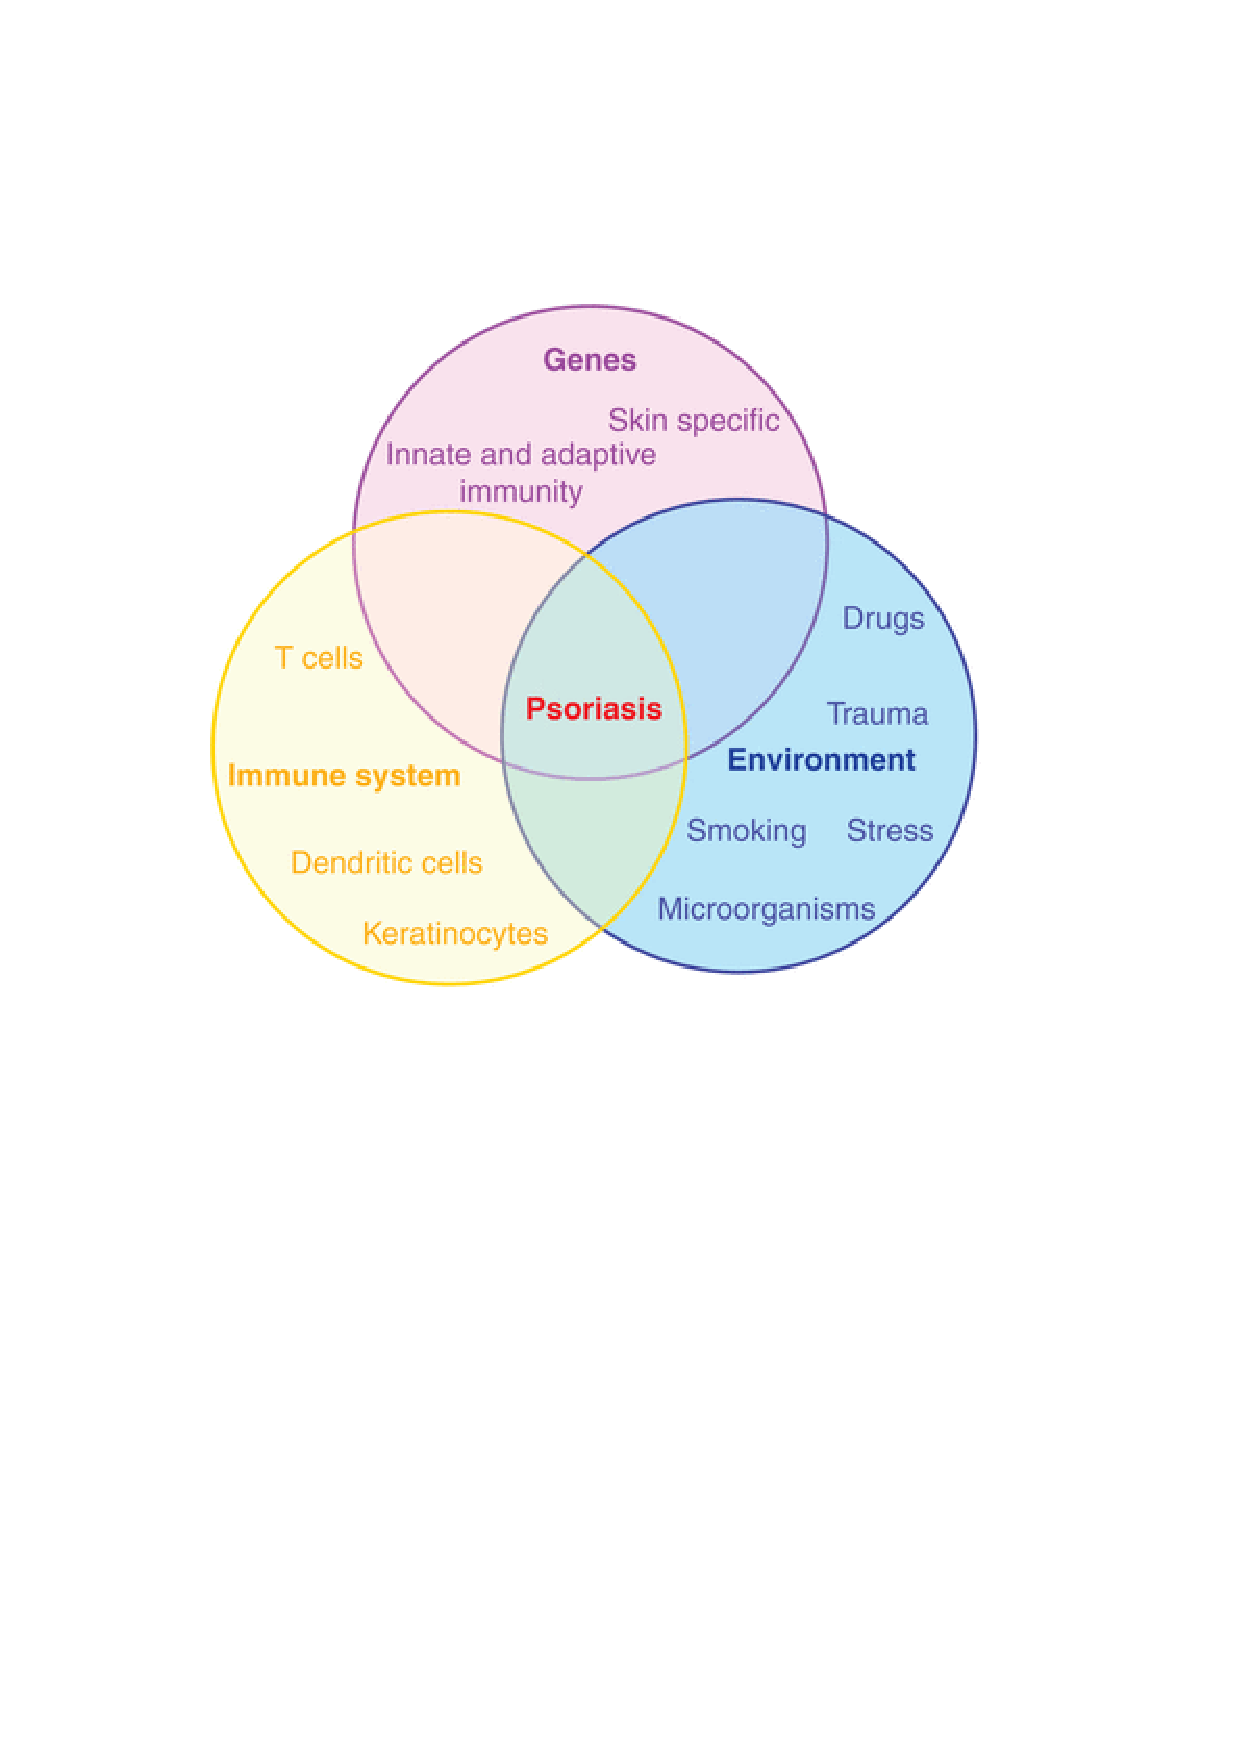
\includegraphics[width=\textwidth]{./Introduction/pdfs/PSO_aetiology_diagram_Di_Meglio_et_al_2014.pdf}
%\caption[Main factors involved in psoriasis disease aetiology]{\textbf{Figure adapted from \parencite{Meglio2014}}}
%\label{fig:PSO_aetiology_diagram}
%\end{figure}

\subsubsection*{Environmental factors and disease}

A variety of exposures are proposed as risk factors for the development and worsening of psoriasis and PsA, with controversy about which are really accountable for disease onset or relapse. A wide range of drugs including anti-depressants, anti-hypertensives and anti-cytokine therapies (e.g $\beta$-blockers and IFN-$\alpha$, respectively) have been associated with initiation, exacerbation and worsening of psoriasis \parencite{Kim2010}. Bacterial and viral infections are associated with triggering and exacerbation of psoriasis and PsA. Onset of guttate psoriasis is associated with throat infection of group C \textit{Streptococcus} and infection with humman immunodefficiency virus (HIV). In PsA statistical association with antibody production against \textit{Streptococcus pyogenes}, \textit{Yersinia enterocolitica}, \textit{ Chlamydophila psittaci} and HIV has also been reported \parencite{Gudjonsson2003,Valdimarsson2009,Diluvio2006,Thrastardottir2018}. Moreover, recent studies have also observed perturbation in the composition of the gut and skin microbiota in both pathologies \parencite{Eppinga2014, Yan2017}.

Physical trauma and mechanical stress can also trigger the appearance of skin lesions and digit joint inflammation \parencite {Weiss2002,Nestle2009}. Increased risk of PsA onset amongst psoriasis patients was indeed associated with lifting cumulative heavy loads as well as with several types of injuries and infections that require treatment with antibiotics \parencite{Eder2011}. Smoking has been the behavioral factor most confidently associated with psoriasis, particularly with palmoplantar pustulosis \parencite{Armstrong2014}. Psoriasis has also shown association with obesity, alcohol dependency, vitamin D deficiency and stress, but evidence still remains controversial \parencite{Meglio2014}. 

\ToDo{Interestingly, epidemiological data suggests a steady increase in psoriasis and PsA prevalence over the last 30 years, particularly in older age groups \parencite{Springate2017,Organization2016}. This trend may be the result of the increase in frequency of various environmental risk factors over the same period of time (for example prevalence of obesity and beta blockers in patients with myocardial infarction), rather than a consequence of the improvement in diagnosis and access to medical care \parencite{Icen2009}. Altogether this reinforces the role of environmental factors in the risk of developing psoriasis and PsA. }


\subsubsection*{Histopathological alterations in skin and joints}

The epidermis is the most external compartment of the skin, comprising approximately 90\% keratinocytes  and is organised in a layer-like structure that self-renews in a spatial and time-dependent manner \parencite{Wikramanayake2014}. Keratinocyte differentiation is associated with changes in morphology, replication ability and keratin composition of the intracellular matrix. In the context of psoriasis, impaired epidermis cell renewal leads to histological alterations and lesion development. Importantly,  keratinocytes up-regulate their proliferation rate (hyperplasia) causing aberrant cell differentiation (parakeratosis), thickening of the epidermis and scale formation \parencite{Ruchusatsawat2011}. Concomitantly, the skin lesion undergoes hypervascularisation driven by up-regulated expression of angiogenic factors and activation of the endothelium that contributes to immune cell infiltration and inflammation \parencite{Perera2012}.  

% Check content accuracy
In PsA, the affected joint shows a wide range of histological changes, one of the most common being arthritis caused by the swelling and inflammation of the joints \parencite{Haddad2013,Schett2011}. \ToDo{As a result, alterations in bone remodelling lead to osteolysis, bone resorption and erosion at the affected joints \parencite{Mensah2008}. Moreover, 35\% of PsA patients also undergo inflammation of the connective tissue at the insertion of tendons or ligaments, a phenomenon known as enthesitis \parencite{McGonagle2011,Polachek2017}. The inflammatory environment at the entheses favours bone spurs formation along the insertion sites, similar to RA, causing structural debilitation of the joints \parencite{Benjamin2009,Finzel2014}. Interestingly, enthesitis has been identified as the main mechanism driving dactylitis, which is importantly characterised by tenosynovitis of the flexor tendons that are constrained by accessory pulleys (sites of compressive and tensile biophysical stress). The accessory pulleys behave as functional entheses and high-resolution magnetic resonance imaging has shown inflammation of this structure in early dactylitis \parencite{McGonagle2019}.}



\subsubsection*{Dysregulation of the innate and adaptive immune response}
%link to the histological changes
The dysregulated immune response in psoriasis and PsA is the result of the interaction between innate and adaptive immune cells through feedback loops and a complex cytokine milieu (Figure \ref{fig:PSO_immune_system_diagram}). Interferon (IFN)-$\alpha$, $\beta$ and $\gamma$ are innate immune cytokines involved in disease initiation and are produced mainly by circulating plasmacytoid dendritic cells (pDCs), T lymphocytes and natural killer (NK) cells in the lesional skin \parencite{Johnson-Huang2009,Perera2012,Hijnen2013}. Increased mRNA levels for IFN-$\alpha$ and $\beta$ have been detected in skin plaques and shown to contribute to lymphocyte recruitment and maintenance of DC activation \parencite{Schmid1994}. Tumour necrosis factor (TNF)-$\alpha$ is another key cytokine involved in the dysregulated innate immune response observed in psoriasis and PsA. TNF-$\alpha$ is produced by innate immune cells, including mDCs, activated keratinocytes, monocytes/macrophages, NK cells
%include NK reference
 and also cells from the adaptive immune system, including the T helper (Th)/CD4$^+$ activated cell subsets Th-1 and Th-17 present at skin lesions and inflamed joints \parencite{Perera2012,Lizzul2005}. TNF-$\alpha$ causes down-stream activation of the nuclear factor kappa-light-chain-enhancer of activated B cells (NF-$\kappa$B), a master transcriptional regulator which induces expression of pro-inflammatory cytokines, antiapoptotic genes and genes involved in maintenance of chronic inflammation \parencite{Lizzul2005, Johansen2004}. Moreover, TNF-$\alpha$ has a prominent role in bone turnover and bone remodeling (mainly enhancing bone resorption), key histopathological features of PsA \parencite{Mensah2008}. 
 % Johansen 2010 Preferential inhibition of the mRNA expression of p38 mitogen-activated protein kinase regulated cytokines in psoriatic skin by anti-TNF-a therapy. 

Interleukin-23 (IL-23) and interleukine-17 (IL-17) constitute a link between the innate and adaptive immunity as well as a key loop for the perpetuation of the psoriasis and PsA inflammatory response. IL-23 is an innate immune cytokine mainly produced by myeloid DC (mDCs) and, to a lesser extent, by lesional skin-resident macrophages and psoriatic keratinocytes \parencite{Lee2004, Li2018}. IL-23 binds to the IL-23 receptor (IL23R) and is highly expressed by the lesion-resident DCs, and T cells, and also by circulating CD4$^+$ from psoriasis patients  \parencite{Tonel2010}. In psoriasis, IL-23 mediates the pathogenic loop between activated keratinocytes and T cells. Binding of IL-23 to the IL-23R receptor expressed by memory CD4$^+$ and CD8$^+$ T cells leads to their differentiation into Th-17 and Tc-17 cells, both characterised by producing high levels of the IL-17 cytokine that activate NF-$\kappa$B, AP-1 and MAPK signalling, amongst others \parencite{McGeachy2009}. %by \textit{TRAF3IP2} (ref). 
IL-17 signalling maintains the Th-17 immune mediated response through recruitment and activation of neutrophils, induction of pro-inflammatory cytokines, including interleukin-1$\beta$ (IL-1$\beta$) and interleukin-6 (IL-6), and sustained keratinocytes activation \parencite{Doyle2012}.

More recently, interleukin 22 (IL-22) has gained relevance as mediator of dysregulated crosstalk between the innate and adaptive immune response. IL-22 levels are increased in the skin lesions and plasma of psoriatic patients and is mainly produced by a subset of CD4$^+$ cells known as Th-22 \parencite{Wolk2006}. IL-22 contributes to keratinocytes hyperproliferation and their production of antimicrobial peptides (AMPs)  \parencite{Eyerich2009}.

% Maybe a paragraph to connect skin and joint affection Identical T cell clonality between skin and synovium https://ac.els-cdn.com/S0198885999000348/1-s2.0-S0198885999000348-main.pdf?_tid=5efa7316-fde5-11e7-8091-00000aacb360&acdnat=1516454913_dd20efb867f822d68d8b09873601e8ad

\begin{figure}[htb]
\centering
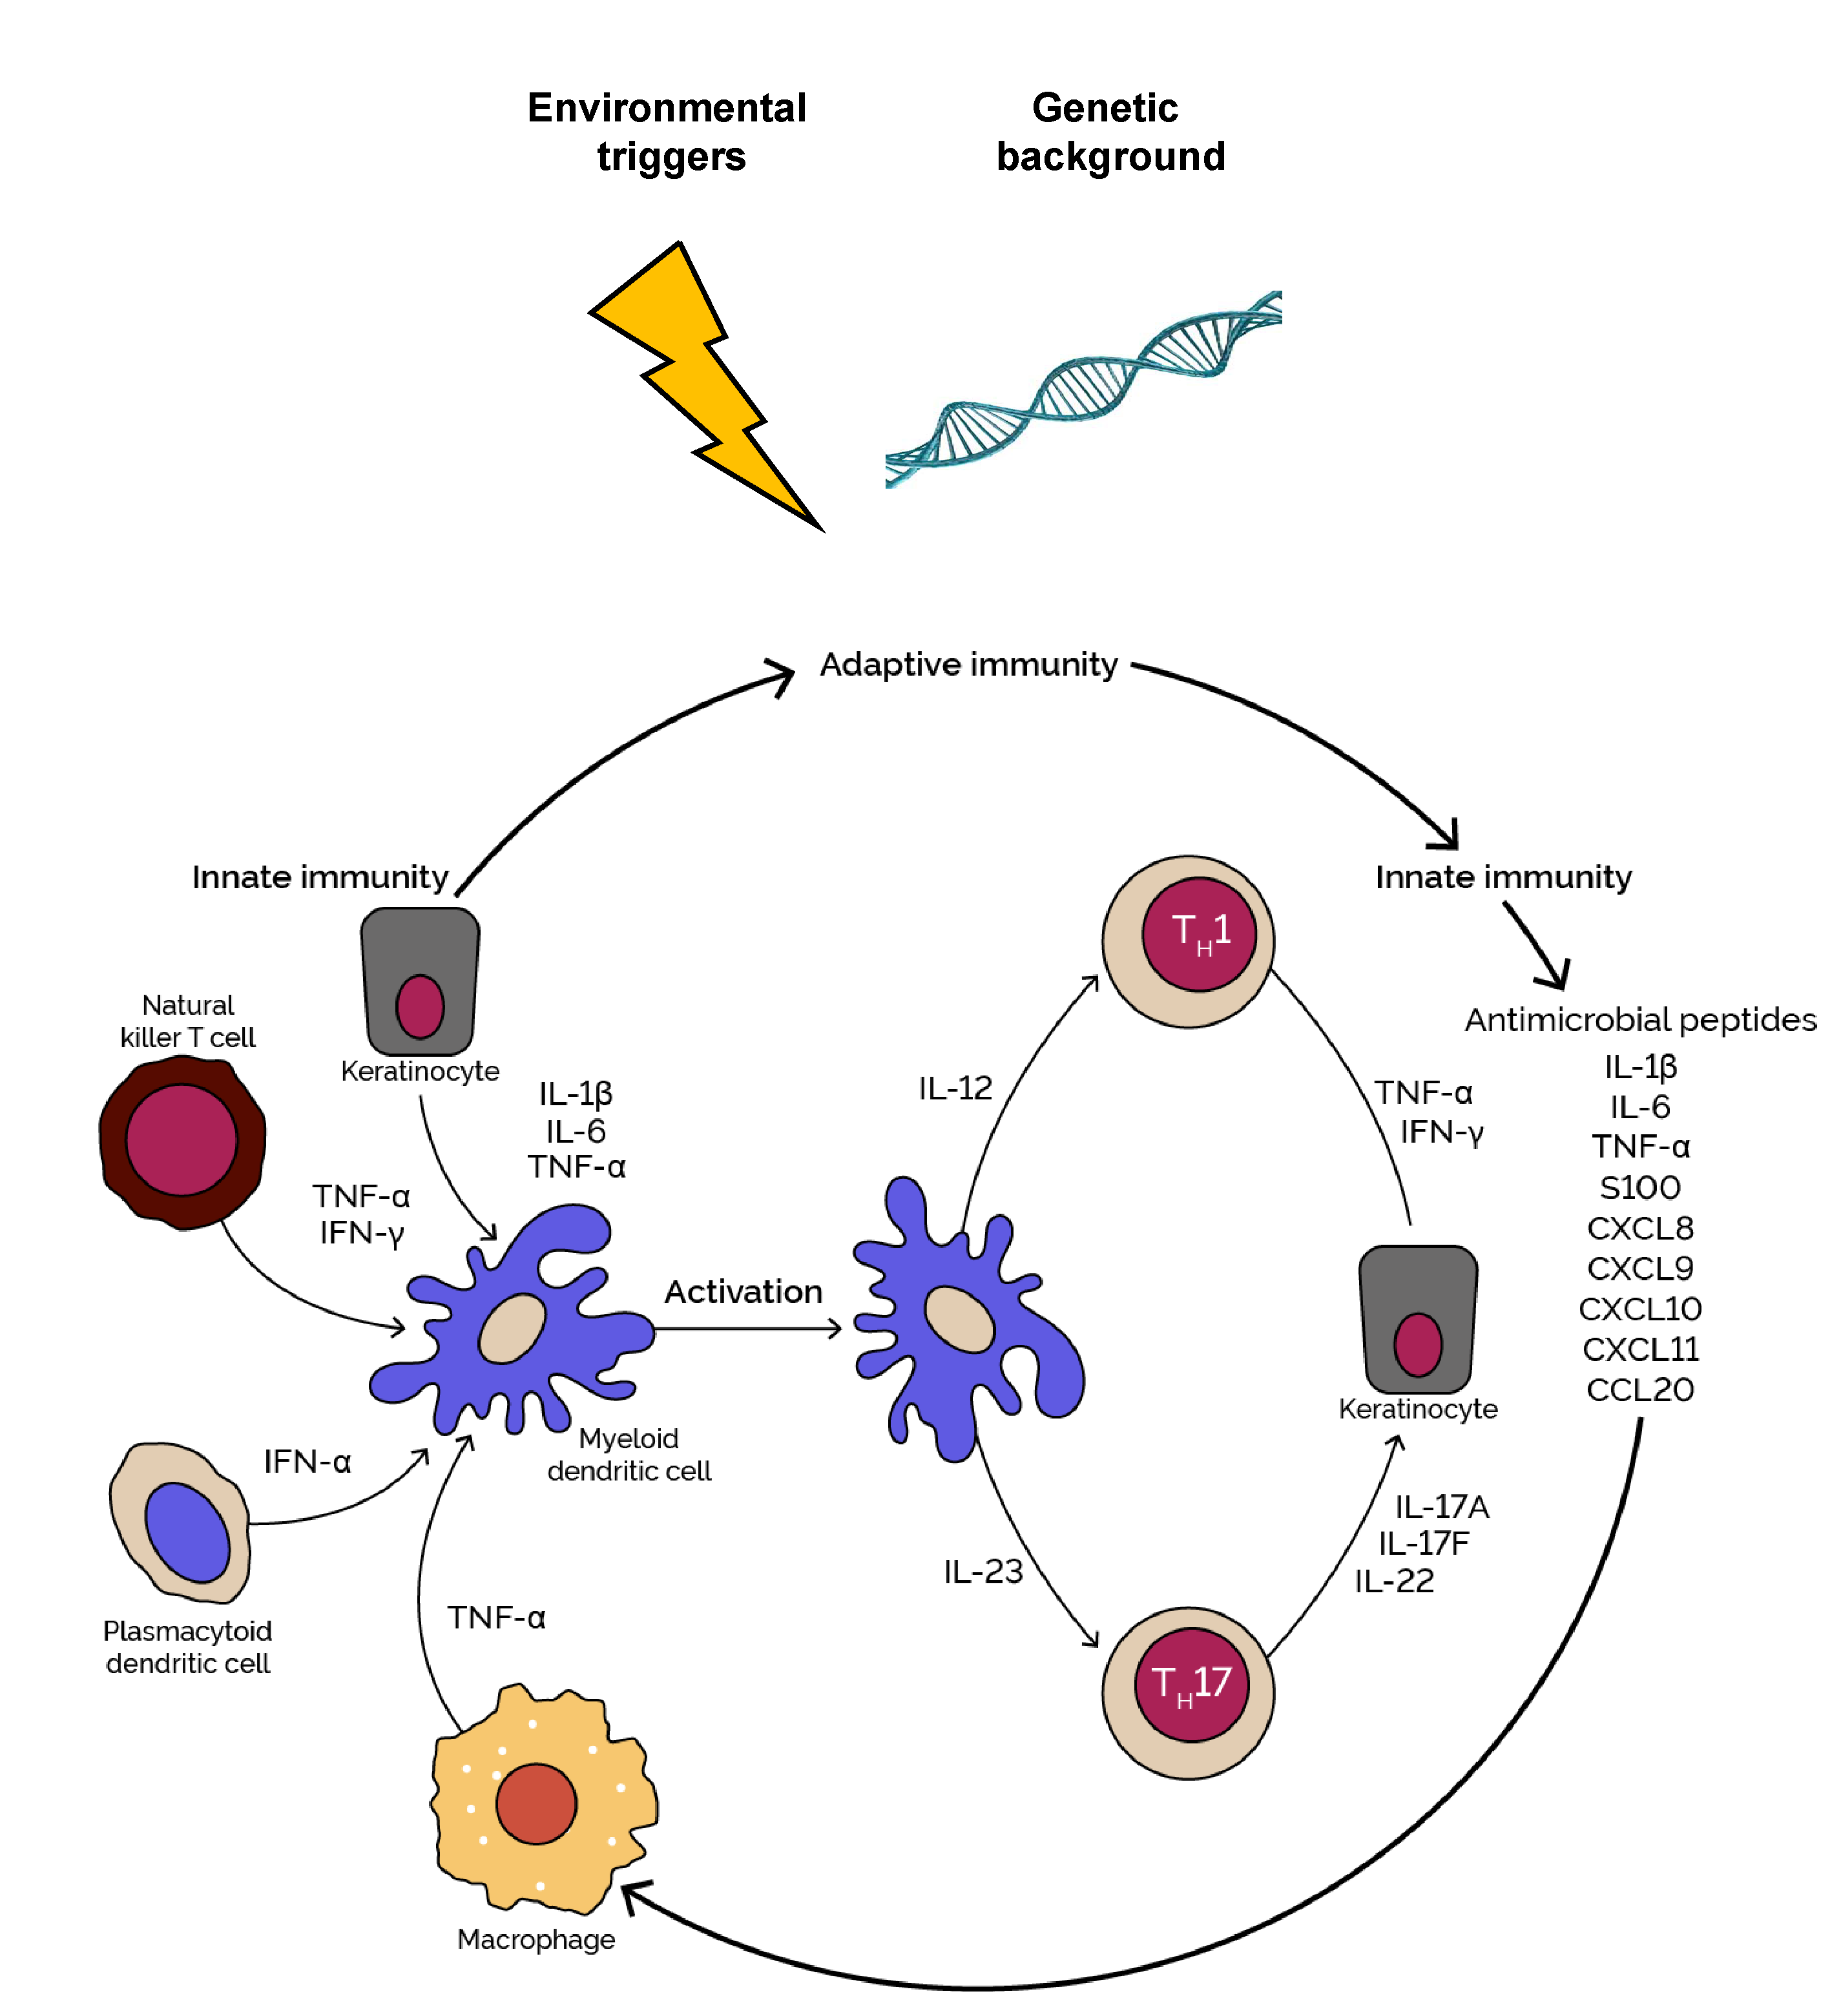
\includegraphics[width=0.7\textwidth]{./Introduction/pdfs/PSO_adaptive_innate_immune_system_crosstalk_new}
\caption[Environmental triggers and genetic predisposition leading to psoriasis and PsA (adapted from Nestle \textit{et al.} 2009).]{\textbf{Environmental triggers and genetic predisposition leading to psoriasis and PsA (adapted from Nestle \textit{et al.} 2009).} The main cell types, cytokines and chemokines involved in the dysregulated innate and adaptive immune response found in these conditions are shown.}
\label{fig:PSO_immune_system_diagram}
\end{figure}

\subsection{Cell types involved in psoriasis and PsA pathogenesis}
%Global report on psoriasis, 2016

Psoriasis and PsA are complex dynamic pathophysiological processes, and the understanding of the relative importance of different cell types at different disease stages still remains challenging.


\textbf{\textit{Keratinocytes}}. In psoriasis, keratinocytes represent a bridge between the innate and adaptive immune response. Keratinocytes have the ability to act as immune sentinels through MHC-class II antigen presentation to CD4$^+$ and also T cytotoxic(Tc)/CD8$^+$ cells through MHC-class I \parencite{Black2007}. Upon damage by environmental triggers, keratinocytes release cationic AMP, such as  LL-37, and self-DNA/RNA that form a complex which acts as an antigen for skin-resident DCs activation and initiation of the inflammatory response \parencite{Lande2007}. Pro-inflammatory cytokines such as IL-17A or IL-22 also induce keratinocyte proliferation and in turn production of cytokines, including IL-1$\beta$, IL-6 and TNF-$\alpha$, and chemokines (e.g CXCL1, CXCL2, CXCL5, CXCL8 and CCL20) leading to recruitment of neutrophils and T cell to the site of inflammation \parencite{Feldmeyer2007, Arend2008, Nestle2009, Nestle2005}. Keratinocytes also release vein endothelial growth factor (VEGF), a pro-angiogenic factor that activates endothelial cells and leads to pathogenic angiogenesis \parencite{Xia2003}. The relevance of keratinocytes in the dysregulated immune response in psoriasis is further reinforced by the genetic association with variants located in keratinocyte-specific genes from the late cornified envelope (LCE) family \parencite{Tsoi2012}. 




\textbf{\textit{Dendritic cells}}. mDCs and pDCs are important innate immune cells in initiation of the psoriasis dysregulated immune response through antigen presentation and T cell activation \parencite{Mahil2016}. pDCs are circulating professional antigen presentation cells (APCs) that infiltrate into the uninvolved and lesional dermis and undergo activation by recognition of self-DNA and LL-37 complex through the Toll-like receptor (TLR)7/9  \parencite{Nestle2005, Lande2007}. This activation prompts the activation and clonal expansion of antigen-specific CD8$^+$ T cells. In contrast, quiescent mDCs are epidermal resident cells that undergo maturation in presence of the IFN-$\alpha$ and $\beta$ secreted by pDCs, expanding up to 30-fold in lesional skin \parencite{Zaba2007}. Activated mDCs mediate the Th-1 and Th-17 response as well as perpetuation of keratinocytes activation through IL-23 , IL-12 and TNF-$\alpha$ production \parencite{Lee2004}. %Studies in immunodeficient psoriasis mouse models have shown that blockage of downstream IFN-$\alpha$ signaling or IFN-$\alpha$ production by pDCs failed to induce T-cell activation and psoriasis onset \parencite{Nestle2005}. 



\textbf{\textit{T cells}}. T lymphocytes have been considered the most relevant cell types in the initiation and maintenance of psoriasis and PsA.  Skin-resident memory T cells have been demonstrated to have a key role in psoriatic lesion development in a mouse model \parencite{Boyman2004}. In human case reports, bone marrow transplantation has been shown to have the ability to both, terminate or initiate psoriasis in recipients \parencite{Gardembas-Pain1990, Eedy1990}. \textit{In vivo} studies demonstrated that transition to psoriatic lesions following engrafted human pre-lesional skin in immune-deficient mice was only dependent on injection of autologous activated CD4$^+$ and not CD8$^+$ cells \parencite{Wrone-Smith1996}. Nevertheless, CD8$^+$ have shown preferential migration into the lesional epidermis where clonal populations have been isolated \parencite{Wrone-Smith1996, Chang1994}. %This may suggest that CD4$^+$ are drivers of T cell activation but resident CD8$^+$ are the main effector cells in the dysregulated psoriasis immune response. 
In psoriasis and PsA, IL-23 together with other cytokines, including IL-1$\beta$ and IL-6, induce activation and differentiation of memory CD4$^+$ and CD8$^+$ into effector pathogenic Th-17 and Tc17 cells producing IL-17 \parencite{Weaver2007}. IL-17$^+$ CD8$^+$ and CD4$^+$ cells have been found in lesional and uninvolved psoriatic skin and are enriched in PsA synovial fluid when compared to peripheral blood, showing correlation with markers of inflammation and structural changes in the joint \parencite{Menon2014,Ortega2009,Lowes2008, Pene2008}. %Additionally, IL-12 and IFN-$\gamma$ lead to expansion of Th-1 and Tc-1 cells, which contribute to perpetuation of the immune response through IFN$\gamma$ and IL-18 production in psoriasis and PsA \parencite{Austin1999, Perera2012}.




%Regarding the adaptive immunity, T lymphocytes have been considered the most relevant cell types in the initiation and maintenance of psoriasis and PsA. Report cases in humans have demonstrated that bone marrow transplantation can initiate or terminate psoriasis \parencite{Eedy1990, Gardembas1990}. Reduced numbers of circulating T cells but increased percentages of the memory populations CD4$^+$CD45RO$^+$ and CD8$^+$CD45RO$^+$ have been observed in moderate-to-severe and severe psoriasis patients when compared to milder phenotypes and healthy controls \parencite{Lecewicz-Torun2001,Langewouters2008}. Different studies have reported controversial results regarding the total abundance and ratios of CD4$^+$ and CD8$^{+}$ in PBMC, likely due to the phenotype heterogeneity of the psoriasis cohorts between studies \parencite{Lecewicz-Toruń2001,Cameron2003,Langewouters2008}. In PsA, no differences in abundance of circulating T cells have been identified when compared to healthy individuals \parencite{Costello1999}.In homeostasis, CD8$^+$ and CD4$^+$ lymphocytes are found in the epidermis and dermis, respectively \parencite{Clark2006}. An increase in activated memory CD4$^{+}$CD45RO$^{+}$and CD8$^{+}$CD45RO$^{+}$ cells can be detected by the third day from the lesion appearance \parencite{Clark2006,Perera2012}. \textit{In vivo} studies showed that development of psoriasis following engrafted human pre-lesional skin was only dependent on local T cell proliferation, highlighting the importance of circulating T cells recruitment during the priming event rather than at later stages of the disease \parencite{Wrone-Smith1996,Nickoloff1999,Perera2012}. The relative importance of CD4$^+$ versus CD8$^+$ cells in psoriasis initiation has been explored in pre-lesional skin mouse xenografts where CD4$^+$ but not CD8$^+$ T cells were required in the transition from uninvolved to lesional skin \parencite{Nickoloff1999}. Interestingly, the injection of activated CD4$^+$ cells in mice was followed by an acute increase in activated resident CD8$^+$ T cells. Overall, these results supported the hypothesis of skin CD4$^+$ cells being drivers of resident T-cell activation and the population of resident activated CD8$^+$ the main effector of the immune response. In synovial tissues of PsA patients, CD4$^+$ are significantly more abundant than CD8$^+$ \parencite{Diani2015}. However, amongst the CD8$^+$ populations, the memory cells are prevalent in the patients’ synovial fluid (SF) with a significant enrichment compared their counterparts in PsA PB and RA SF \parencite{Costello1999}. Based on the cytokine profile, psoriasis and PsA have been classified as a type 1 Th/Tc disease, where activation of naive CD4$^+$ and CD8$^+$ cells is driven by IL-12 and IFN-$\gamma$ \parencite{Austin1999,Perera2012}. In addition, T-cell subsets including Th-17/Tc-17 and Th-22/Tc-22, producing high levels of IL-17 and IL-22, respectively, have been identified to be relevant for the perpetuation of the inflammatory response \parencite{Mahil2016}. The importance of Th-17 cells and IL-17 production has been evaluated in skin, joints and blood, with elevated mRNA and protein levels of IL-17 and also IL-23 reported in psoriasis and PsA patients compared to controls \parencite{Cai2012, Dolcino2015}. %Mention paper Kagami about increased Th17, Th1 and Th22 in psoriasis patients bloodThe relevance of IL-17 has been further highlighted by the presence of CD8$^+$ populations in patients’ SF that are predominantly IL-17 producers and whose abundance correlates with markers of inflammation and structural changes in the joint \parencite{Menon2014}. This finding is in line with observations in skin and suggests a prominent role for CD8$^+$ IL-17-producing cells in the different stages of both pathologies. Studies directed to understand the importance of IL-17 have led to the discovery of other immune cells producing this pivotal cytokine, including innate immune lymphoid (ILC) cells and $\gamma$$\delta$ T cells, opening new research avenues in the context of psoriasis and PsA pathophysiology and treatment \parencite{Meglio2014,Leijten2015}. IL-17-producing cells have also been hypothesised to be at the link between skin and joint lesions. Although the precise mechanisms for transition between psoriasis and PsA is still poorly understood, the study of psoriasis and RA in mouse models revealed that skin lesions facilitate arthritis and joint inflammation \parencite{Yamamoto2015}. %In fact, the presence of IL-17-producing cells in the inflamed skin nearby the enthesis of joints under physical stress is likely to be a trigger for the development of PsA.


\textbf{\textit{Monocytes and macrophages}}. Resident macrophages in the healthy dermis undergo a 3-fold increase in psoriatic skin lesions and contribute to disease development through TNF-$\alpha$ production \parencite{Perera2012, Mahil2016}. Similarly, a mouse model for chronic psoriasiform skin inflammation has demonstrated macrophage migration into affected skin and how production of TNF-$\alpha$ contributes to maintenance of skin lesions \parencite{Stratis2006, Wang2006}. Initial studies showed greater phagocytic and bactericidal activity in monocytes from psoriasis patients compared to those from healthy individuals \parencite{Bar-Eli1979}. Additionally, increased circulating intermediate-like monocytes (CD14$^{high}$ CD16$^{high}$) and monocyte aggregation was also observed in psoriasis patients, resulting in enhanced platelet activation and angiogenesis \parencite{Golden2015}. In PsA synovial membranes, the levels of monocytes/macrophage secreted metalloproteinases responsible for bone erosion upon differentiation into osteoclasts have been found to be similar to those in RA joints \parencite{Hitchon2002}. Moreover, decreased number of macrophages in PsA synovial tissue have been observed following therapy and proposed as a biomarker to assess treatment response \parencite{Canete2010}.

\textbf{\textit{Natural killer cells}}. NK cells are lymphoid-derived innate immune cells identified as CD3$^-$ CD56$^+$. The majority of circulating NK cells (90\%) are CD56$^{dim}$ and show strong cytotoxicity \parencite{Mandal2015}. In contrast, CD56$^{bright}$  commonly infiltrate into second lymph organs and other tissues, where they are activated by DCs and produce immunoregulatory cytokines such as IFN-$\gamma$, CCL5, CCL3 and GM-CSF that contribute to the shaping and regulation of other immune cells and promote Th-1 expansion and activation of the adaptive immune response \parencite{Martin-Fontecha2004,Ferlazzo2004}. In psoriasis, a significant increase of cells expressing NK markers have been found in lesional compared to uninvolved skin \parencite{Cameron2003,Ottaviani2006}.  %with NK CD56$^{bright}$ cells isolated from acute plaque lesions producing abundant IFN-$\gamma$ upon activating stimuli \parencite{Cameron2002,Ottaviani2006}. 
 In a cohort including RA, PsA and AS patients, expansion of NK CD3$^-$ CD56$^{bright}$ cells was observed in inflamed joints \parencite{Dalbeth2002}. Moreover, NK cells in RA have shown to trigger osteoclastogenesis and bone destruction \textit{in vitro} and also in mice \parencite{Soederstroem2010}. %Moreover, the cytokine IL-15, which is highly present in the the joint microenvironment can prime NK cells isolated from PsA peripheral blood to kill via activation of the receptor NKG2D and cPLA2.82 \parencite{Tang2013}. 
Additionally, the NK receptors from the killer immunoglobulin-like receptor (KIR) family KIR2DL1 and KIR2DS1 (inhibitory and activatory, respectively) recognise HLA-Cw*06:02, strongly associated with psoriasis and PsA \parencite{Tobin2011}. In fact, gene based studies have shown genetic variability in \textit{KIR2DS1} associated with psoriasis and PsA susceptibility, as well as with AS and RA \parencite{Luszczek2004, Williams2005,Carter2007,Yen2001}


\textbf{\textit{Neutrophils}}. Neutrophils are implicated in disease initiation through their ability to form neutrophil extracellular traps (NET) that contain host DNA and LL-37 \parencite{Hu2016}. Evidence of increased NET formation in peripheral blood and lesional skin of psoriasis patients has been found and seems to contribute to pDC and CD4$^+$ T cell activation \parencite{Hu2016}. Neutrophils have also been identified as one of the main sources of IL-17  in skin lesions and to release a wide range of proteases, some of which induce keratinocyte proliferation \parencite{Lin2011,Mahil2016}.
%Add chemokines


%HLA-Cw*06:02 can be recognised by the inhibitory receptor KIR2DL1 and the activatory receptor KIR2DS1.  Some studies have shown KIR2DS1 was present in 85\% of the patients but only in 51\% of the controls
%NK cells are important regulators of immune responses \parencite{Luszczek2004}. Their function extends beyond killing of infected or transformed cells. Interactions with dendritic cells, macrophages, and fetal trophoblast cells can regulate NK cell activity by influencing cytokine production, cytotoxicity and stimulation of T helper-1 responses. 
%
%

\textbf{\textit{B cells}}. B cells are mainly involved in the humoral adaptive immune response through antibody production. However, they also act as APCs, regulate CD4$^+$ activation and differentiation into Th effector cells by providing coestimulatory signals and actively secrete cytokines \parencite{Bouaziz2007,Constant1995,Harris2000,Linton2003}. The role of B cells in the pathophysiology of psoriasis and PsA remains unclear since both are negative for auto-antigens. Recent studies on the imiquimod-induced psoriasis mouse model have demonstrated a more severe inflammation in CD19$^{-/-}$ knock-out mice lacking a regulatory B cell subset producing IL-10 \parencite{Yanaba2013,Alrefai2016}. Furthermore, different B cell subsets have been found in PBMCs from psoriasis patients and in lesional skin, and correlation with disease severity has been identified for some clinical subtypes \parencite{Lu2016}. Moreover, enrichment of psoriasis GWAS risk SNPs in B cells regulatory elements \parencite{Farh2015, Patrick2018}.





\subsection{Therapeutic intervention}
Psoriasis and PsA are currently incurable diseases, with available treatments focused on alleviating symptoms. For instance, topical therapies are advocated in cases of mild-to-moderate psoriasis, including emollients and short-term corticosteroids \parencite{Menter2009}. Other treatments may be used in combination with corticosteroids, such as ultraviolet (UV) light therapy and vitamin D analogues, directed to inhibit T-cell and keratinocyte proliferation and also induce keratinocyte differentiation \parencite{Rizova2001}. In the case of PsA, for patients presenting with swelling of two or fewer joints, nonsteroidal anti-inflammatory drugs (NSAID) and intra-articular injection of glucocorticosteroids, together with joint aspiration, are used to reduce pain and inflammation \parencite{Coates2016}. 

Treatment of most forms of PsA and moderate-to-severe psoriasis requires the use of systemic therapies. More severe forms of PsA require disease-modifying antirheumatic drugs (DMARDs) including antagonist of folic acid methotrexate and phosphodiesterase 4 inhibitor Apremilast, which act as immunosuppressors of activated T cells and cytokine production, respectively \parencite{Schmitt2014, Gossec2016, Keating2017,Polachek2017}. Biologic systemic agents represent the most specific treatment option for severe psoriasis and PsA notably TNF-$\alpha$ inhibitors (TNFi). Three TNFi have been approved for the treatment of psoriasis: etanercept, infliximab and adalimumab \parencite{Mahil2016}. In addition, certolizumab pegol and golimumab are often used in the management of PsA \parencite{Coates2016a}. However, side effects of TNFi such as increased risk of infection or reactivation of latent infections have been identified \parencite{Gottlieb2003}. Moreover, 20 to 50\% of patients fail to respond to the first TNFi administrated, requiring switching to an alternative TNFi \parencite{Abramson2016}. New biologic therapies have been developed to target other key cytokines, such as IL-12, IL-23 (ustekinumab) or IL-17 (secukinumab and ixekizumab), which represent a substantial advance in treating patients failing to respond to TNFi \parencite{Mahil2016, Coates2016a}.

% Bispecific antibodies

 

\section{Genetics of psoriasis and psoriatic arthritis}

\subsection{Heritability}

\ToDo{The risk of developing psoriasis and PsA is not only influenced by environmental conditions but also by the genetic background of each individual. In fact, approximately 40\% of patients with psoriasis or PsA have a family history in first degree relatives \parencite{Gladman1986}. Twins studies in patients with psoriasis (only cutaneous lesions) have demonstrated that concordance of disease is greater in monozygotic (33-55\%) compared to dizygotic twins (13-21\%), giving a heritability estimate between 50 to 80\% in populations of European descendants \parencite{Farber1974, Duffy1993,Grjibovski2007,Pedersen2008,Lonnberg2013}. Moreover, psoriasis prevalence is also greater amongst first degree relatives compared to the general population, ranging between 4-19\% \parencite{Myers2005,Chandran2009}.} 

\ToDo{Interestingly, the only twins study conducted to date in PsA did not find differences in concordance between monozygotic and dizygotic twins, which could be due to lack of power in the study \parencite{Pedersen2008}. Nevertheless, heritability estimates in PsA are between 80 to 100\% and the recurrence rate in first-degree relatives has been shown to be greater for PsA (40-47-fold) compared to psoriasis (8-fold) \parencite{Myers2005,Chandran2009,Karason2009}. These observations may highlight differences in the heritability between the two phenotypes and a stronger genetic contribution in PsA compared to psoriasis.}





%\subsection{Non-GWAS and linkage studies}

%Linkage analysis of psoriasis and PsA in family pedigrees presenting an autosomal dominant condition yielded nine psoriasis susceptibility loci (PSORS1-9) with PSORS1 showing the strongest genetic association \parencite{Capon2017, Consortium2003}. PSORS1 locus lies within the MHC class I region, initially associated with psoriasis susceptibility in serological studies \parencite{Russell1972, Tiilikainen1980}. Rare highly penetrant mutations have also been identified for two genes within PSORS2 (17q25): zinc finger protein 750 (\textit{ZNF750}) and caspase domain family member 14 (\textit{CARD14}), with common variants in \textit{CARD14} also reported in psoriasis and PsA patients, implicating genetic variation in this gene in Mendelian and multi-factorial forms of disease \parencite{Tomfohrde1994,Jordan2012, Jordan2012a,Tsoi2012}. Nevertheless, the inability of independent studies to reproduce these results for regions other than PSOR1, 2 and 4, highlights the limitations of linkage studies to understand the genetics of complex diseases \parencite{Capon2017}. 



%Additionally, gene based studies in psoriasis and PsA disclosed the importance of genetic variability in the activating killer immunoglobulin receptors 2DS1 (\textit{KIR2DS1}) gene, also reported for AS and RA, which interestingly is mainly triggered by interaction with HLA-Cw*06:02 \parencite{Luszczek2004, Williams2005,Carter2007, Yen2001}.  
%Similarly, specific association with PsA but not psoriasis was found for microsatellites and promoter polymorphisms in TNF-$\alpha$ \parencite{H\"{o}hler2002}. 


\subsection{Genome-wide association studies}
\label{GWAS}

Initially, linkage studies were used to dissect the genetic architecture of psoriasis and PsA. A susceptibility loci in chr16p was identified by linkage analysis in families with PsA, suggesting a role of imprinting and paternal transmission \parencite{Karason2003}. A study of psoriasis in family pedigrees presenting an autosomal dominant condition revealed nine psoriasis susceptibility loci (PSORS1-9) with PSORS1 showing the strongest genetic association \parencite{Consortium2003}. Nevertheless, the inability of independent studies to reproduce these results for regions other than PSOR1, 2 and 4 highlighted the limitations of this approach to understand the genetics of complex diseases \parencite{Capon2017}.

Advances in the ability to catalogue genome-wide common single base-pair changes known as single nucleotide polymorphisms (SNPs) led to the implementation of genome-wide association studies (GWAS). GWAS are focused on identifying disease-associated common SNPs (with minor allele frequency (MAF)$\geq$1 to 5\% ), showing differences in allele frequency between patients and controls \parencite{Ku2010}. GWAS are thus based on the hypothesis that complex diseases are caused by the interaction of multiple common variants, with modest effect size, with OR between 1.2 and 2 \parencite{Schork2009, Cui2010}. The genotyped SNPs in GWAS are used as a proxy for the disease causative variant, which can be non-genotyped SNPs or copy number variants (CNVs) \parencite{Hirschhorn2005, Ku2010}.

%Due  to the organisation of the genome into segments of strong linkage disequilibrium (LD) where genetic variants are strongly correlated with each other, the genotyped SNPs in GWAS are solely used a proxy for the disease causative variant. Therefore, disease causal variants can be non-genotyped SNPs or other type of genetic variability such as copy number variants (CNVs), also highly frequent in the genome but less widely studied by GWAS \parencite{Hirschhorn2005, Ku2010}. 

\ToDo{The first psoriasis GWAS published in 2007 by Cargill \textit{et al.} has been followed by other studies with larger sample sizes and meta-analysis across different cohorts (Table \ref{tab:GWAS_summary}). The vast majority of these GWAS have combined psoriasis (only cutaneous lesions) and PsA patients in the cases group. Up to date, psoriasis GWAS studies have identified a total of 63 independent associations at genome-wide significance (p-value$<$5x10$^{-8}$) in European population, which only account for 28\% of the overall estimated psoriasis and PsA heritability  \parencite{Tsoi2017}. The majority of studies have been performed in Caucasian European or North American cohorts, but increasing numbers of GWAS in large Chinese cohorts are also being published, increasing the number of independent associated loci to 70 \parencite{Zhang2009, Sun2010, Yin2015}. Early GWAS with moderate power confirmed association with loci overlapping the PSOR1 and PSOR2 genomic regions  \parencite{Cargill2007,Strange2010}.} 


\ToDo{The informativeness of GWAS was significantly enhanced with the use of the Immunochip genotyping chip, which covers 186 immune relevant loci identified in previous GWAS across different inflammatory diseases at a greater genotyping density \parencite{Tsoi2012}. The psoriasis Immunochip study uncovered 15 new associations, including \textit{CARD14} at the PSOR4, and also performed a meta-analysis incorporating the largest available psoriasis cohorts at the time \parencite{Tsoi2012}. This meta-analysis has since been further expanded, yielding sixteen additional associations and reinforcing the importance of NF$\kappa$B and cytotoxicity pathways in disease pathophysiology \parencite{Tsoi2015a,Tsoi2017}. Meta-analysis of GWAS across Caucasian and Chinese populations revealed four new associations as well as population-specific effect or allelic heterogeneity in eleven loci (including MHC-I genes), demonstrating the value of a trans-ethnic approach to further understand the heterogeneous genetic susceptibility to psoriasis in different populations \parencite{Yin2015}. }
%Four new non-coding loci in the vicinity of \textit{LOC144817}, \textit{COG6}, \textit{RUNX1} and \textit{TP63} were associated with psoriasis and PsA in both populations. Interestingly, genetic heterogeneity between Caucasian and Chinese cohorts was also observed for ten of the GWAS reported loci, for example \textit{ELMO1} and \textit{TYK2}.


\subsubsection{Non MHC genome-wide associations in psoriasis and PsA}

\ToDo{A limited number of PsA GWAS have been conducted,being the best powered the Immunochip study performed by Bowes and colleagues \parencite{Liu2008,Huffmeier2010,Ellinghaus2012a,Bowes2015}. These studies identified a total of thirteen PsA associated loci at genome-wide significance (p-value$<$5x10${-8}$).  The  Immunochip PsA GWAS also unveiled PsA-specific associations at the  \textit{IL23R}, 5q31 and \textit{PTPN22} loci, which did not show significant associations (not even at nominal p-value$<$0.05) in psoriasis patients \parencite{Bowes2015, Bowes2015a}. } 
\ToDo{Following the Immunochip PsA GWAS, Stuart and colleagues published a larger study than the one conducted in 2010, comparing associations between PsA patients and those psoriasis patients with skin symptoms that had not developed PsA for at least ten years (Table \ref{tab:GWAS_summary}). This study revealed nine regions associated with PsA (\textit{IFNLR1},\textit{IL23R}, \textit{REL},\textit{IFIH1},\textit{TNIP1}, \textit{IFNLR1}, \textit{IL12B}, \textit{TRAF3IP2}, \textit{NFKBIA} and \textit{TYK2}) and ten with cutaneous psoriasis (\textit{TNFRSF9}, \textit{LCE3C/B}, \textit{IL13}, \textit{TNIP1}, \textit{IL12B}, \textit{TRAF3IP2}, \textit{TNFAIP3}, \textit{IL23A}, \textit{NFKBIA} and \textit{NOS2}) at genome-wide significance. 
Amongst the psoriasis (combined cutaneous psoriasis and PsA together) GWAS variants reported by Stuart and colleagues, those nearby \textit{TNFRSF9} and \textit{LCE3A} showed stronger association with cutaeous psoriasis than PsA whereas variants at the \textit{IL23R} and \textit{TNFAIP3} loci presented stronger association with PsA compared to cutaneous psoriasis. Moreover,the PsA significantly associated variants at \textit{IL23R} (previously reported by Bowes \textit{et al.}, 2015) and \textit{TNFAIP3} loci were independent from previously identified psoriasis variants at the same loci.} 

\ToDo{Interestingly, PsA-specific signals previously identified by less powered studies failed to show significant differences in association between cutaneous psoriasis and PsA in the Stuart and colleagues analysis (including the 5q31 loci reported by the Immunochip PsA GWAS), and only the \textit{PTPN22} locus reached nominal stronger association in PsA \parencite{Stuart2015}. The latest phenotype-specific association analysis published by Patrick and colleagues in 2018 has increased the number of genome-wide association with PsA and cutaneous psoriasis to thirteen and fifteen, respectively, with all of these loci previously identified as psoriasis associated  \parencite{Patrick2018}.}




\subsubsection{Differences in  the MHC associations between psoriasis and PsA}
\ToDo{Regarding MHC associations with psoriasis, \textit{HLA-Cw*06:02} has been consistently identified as the most significantly associated locus with the greatest effect size in psoriasis and also in independent analysis of cutaneous psoriasis and PsA compared to controls \parencite{Okada2014, Bowes2015,Stuart2015}. Step-wise conditional analysis has revealed additional HLA-I and HLA-II associations, including \textit{HLA-C*12:03}, HLA-B amino acid positions 67 and 9, HLA-A amino acid position 95, and HLA-DQA1 amino acid position 53, with similar results found in the independent analysis of cutaneous psoriasis and PsA compared to controls \parencite{Okada2014, Bowes2015}. }

\ToDo{Dissecting the \textit{HLA-Cw*06:02} association in psoriasis and PsA has remained challenging. \textit{HLA-Cw*06:02} has been demonstrated to increase risk of PsA when compared to controls. However, in the comparison between cutaneous psoriasis and PsA \textit{HLA-Cw*06:02} appeared as more strongly associated with cutaneous psoriasis and showed a protective effect for PsA within psoriasis \parencite{Whinchester2012,Eder2012, Stuart2015}. %In addition to HLA-Cw*06:02, Okada and colleagues reported HLA-B aminoacis 45 to be the driver of the stronger association in PsA compared to psoriasis. 
Since \textit{HLA-Cw*06:02} is also associated with earlier age of onset in psoriasis, accounting for age of onset in the comparison of cutaneous psoriasis vs PsA \textit{HLA-Cw*06:02} did not show protective association in PsA \parencite{Bowes2017}. Instead the most significant MHC association when comparing both phenotypes was HLA-B aminoacid 97 (asparagine, mostly found in HLA-B*27),  which differentiated PsA from cutaneous psoriasis \parencite{Bowes2017}.}



%
\begin{landscape}
\begin{center}
\renewcommand{\arraystretch}{0.7}	
\begin{longtable}[ht]{p{.25\textheight} p{.25\textheight} p{.20\textheight} p{.20\textheight} p{.50\textheight}}
%{p{.15\textheight} p{.15\textheight} p{.25\textheight} p{.25\textheight} p{.15\textheight} p{.15\textheight} p{.15\textheight}}
\caption[Main GWAS in psoriasis and PsA]{\textbf{Main GWAS in psoriasis and PsA.} Summary table describing the most relevant psoriasis and PsA GWAS. Information regarding sample size, patients phenotypes and the main reported associations in each study is included. The Stuart \textit{et al.} 2010, Stuart \textit{et al.} 2015 and Patrick \textit{et al.} 2018 studies included stratified association analysis of cutanous psoriasis (patients with skin symptoms that had not developped PsA for at least ten years) and PsA independently. WA=white American; Eur=European; $^\star$ Meta-analysis performed.}
\label{tab:GWAS_summary} \\
\toprule
\textbf{Study} & \textbf{Etnicity} & \textbf{Sample size}      & \textbf{Phenotype} & \textbf{Main associations} \\
               &                   & \textbf{(Cases/Controls)} &                    &  \textbf{(putative genes)}                  \\
\midrule
\midrule
\parencite{Cargill2007} &	WA &	1,446/1,432 & Psoriasis(+PsA) &	HLA-C (PSOR1) and \textit{IL-12B} \\
\parencite{Nair2009} &	Eur	& 1,409/1,436 &	Psoriasis(+PsA) &	\textit{IL-23A}, \textit{IL23R}, \textit{IL-12B}, \textit{TNIP1}, \textit{TNFIP3}, \textit{IL-4} and \textit{IL-13} \\
\parencite{Stuart2010} &	WA, Eur &	1,831/2,546	& Cutaneous psoriasis, PsA &	\textit{NOS2}, \textit{FBXL19},\textit{PSMA6-NFKBIA} \\

\parencite{Ellinghaus2010} &	German	& 472/1,146	& Psoriasis (skin only) & \textit{TRAF3IP2} \\

\parencite{Strange2010} &	Eur & 2,622/5,667 & Psoriasis(+PsA) & \textit{LCE3D} (PSOR2), \textit{IL28RA}, \textit{REL}, \textit{IFIH1}, \textit{ERAP1}, \textit{TYK2} and \textit{HLA-C/ERAP1} epistasia \\

\parencite{Zhang2008} & Chinese	& 1,139/1,132	& Psoriasis (type I)  & \textit{LCE} gene family and \textit{IL-12B} \\

\parencite{Sun2010} & Chinese	& 8,312/12,919	& Psoriasis(+PsA) &	\textit{ERAP1}, \textit{PTTG1}, \textit{CSMD1}, \textit{GJB2}, \textit{SERPINB8} , \textit{ZNF816A} \\

\parencite{Tsoi2012}$^\star$ & WA, Eur & 10,588/22,806 & Psoriasis(+PsA) & \textit{CARD14} (PSOR4), \textit{RUNX3}, \textit{B3GNT2}, \textit{ELMO1}, \textit{STAT3} \\

\parencite{Tsoi2015a}$^\star$	& WA, Eur	& 15,000/27,000	& Psoriasis(+PsA)	& 1q31.1, 5p13.1, \textit{PLCL2}, \textit{NFKBIZ}, \textit{CAMK2G} \\

\parencite{Bowes2015} &	British, Irish, Australians	& 1,962/8,923	& PsA	& 5q31 PsA-specific \\

\parencite{Stuart2015} &	WA and Eur	& 1,430/1,417	& Cutaneous psoriasis, PsA	& PsA-specific secondary signals (main text), new psoriasis-specific (\textit{CDKAL1} and \textit{CAMK2G}), stronger psoriasis \textit{LCE} association\\

\parencite{Yin2015} &	WA, Eur, Asian	&  15,369/19,517 & Psoriasis(+PsA)	& \textit{LOC144817}, \textit{COG6}, \textit{RUNX1} and \textit{TP63}; signals with ethnic heterogeneity \\

\parencite{Tsoi2017}$^\star$ &	WA, Eur	& 19,032/39,498	& Psoriasis(+PsA)	& \textit{CHUK}, \textit{IKBKE}, \textit{FASLG}, \textit{KLRK1}, \textit{PTEN} \\	

\parencite{Patrick2018} &	WA, Eur	& 11,024/16,336	& Cutaneous psoriasis, PsA	& Thirteen and fifteen loci associated with PsA and cutaneous psoriasis, respectively \\																		
\bottomrule
\medskip
\end{longtable}
\end{center}
\end{landscape}


\ToDo{Overall, GWAS have demonstrated shared and distinct genetic architectures in MHC and non-MHC loci between cutaneous psoriasis and PsA, adding a layer of complexity in the understanding of the similarities and differences bewteen the two pathologies.}


\subsection{Relevance of non-coding variants in disease susceptibility}

Approximately 88\% of all GWAS associations map within non-coding regions \parencite{Welter2013}. Psoriasis exome association studies in Chinese and Caucasian populations have increased the number of coding variants with putative effects on the protein structure \parencite{Tang2014, Zuo2015, Dand2017}. These studies have confirmed some previously identified missense associations in \textit{CARD14} and \textit{ERAP1}, revealed new common coding variants at these previously associated loci and identified rare protective missense changes, for example in the \textit{TYK2} gene \parencite{Tang2014,Dand2017}. Nevertheless, results from extensive exome studies suggest that non-synonymous SNPs have a limited contribution to the overall genetic risk of psoriasis compared to non-coding variants \parencite{Tang2014}.

Efforts have been made to elucidate the association of non-coding variants to disease by their ability to regulate gene expression in a cell and context specific manner  \parencite{Fairfax2012, Fairfax2012, Naranbhai2015,Nica2011}. Susceptibility variants can be located in different regulatory elements, including enhancers, silencers, promoters and the 5' and 3' untranslated regions (UTRs)  \parencite{Ward2012}. Non-coding GWAS variants can alter the expression of target genes through different mechanisms including changes in chromatin accessibility, histone modifications, protein binding such as transcription factors (TFs), DNA methylation and binding of non-coding RNA molecules \parencite{Knight2014} (see \ref{subsec:Epigenetics}).

Identification of the target genes regulated by non-coding variants poses a challenge in the field of functional genetics. This limitation can be partially addressed by conducting expression quantitative trait loci (eQTL) analysis, which identifies genome-wide statistical associations between gene transcript levels and SNPs in \textit{cis} ($<$1Mb) or \textit{trans} to the gene. For instance, in T2D this approach revealed a \textit{cis}-eQTL involving the TF \textit{KLF4} and a haplotype of non-coding GWAS SNPs located 14kb upstream \parencite{Small2011}. Moreover, this haplotype also showed association with genes in \textit{trans}, highlighting indirect downstream targets regulated by KLF4. Nonetheless, eQTL mapping alone only provides statistical suggestion of transcriptomic regulation, and additional functional assays, such as chromatin conformation and genome editing, are required to demonstrate causality \parencite{Edwards2013}.  
 


\subsection{The role of GWAS in highlighting immune-relevant cell types and pathways}

GWAS represent a biologically unbiased approach to shed light on pathophysiologically relevant cell types and molecular pathways associated with disease. The functional relevance and cell-type specificity of GWAS variants can be interrogated by overlapping them with epigenetic features mapped in cell lines or primary cells isolated from healthy controls \parencite{Farh2015}. In psoriasis and PsA, enrichment of associated variants for regulatory elements has been found in several cell types (e.g Th-1 and Th-17 cells) and the majority of GWAS risk loci have been linked to genes from a limited number of pathways, as detailed below \parencite{Tsoi2017,Capon2017}. Most of these genes are reported based on proximity to the associated variants and fail to take account of long-range gene regulation, which represents a limitation when interpreting GWAS results. Additional criteria has also been used to link non-coding GWAS variants to a target gene, including LD with a deleterious variant, direct functional characterisation of the regulatory element and/or genetic variant or association of gene expression with the genotype of the GWAS lead SNP \parencite{Capon2008,Tsoi2012,Tsoi2017,Meglio2011}.

Systematic comparison of the genetic architecture across different diseases revealed that loci associated with psoriasis and PsA are shared in the same or opposite directions, with AS, Crohn’s disease (CD), multiple sclerosis (MS), RA or type 1 diabetes (T1D) \parencite{Tsoi2012}. This has also supported the use of therapeutics such as anti- TNF, IL-23 and IL-17 antibodies across a number of immune-related phenotypes \parencite{Visscher2017}.
%including psoriasis, PsA, AS and IBD, amongst others 





%GWAS represent a biologically unbiased approach to shed some light on pathophysiological relevant cell types and molecular pathways associated with disease. In the field of common immune-mediated diseases, GWAS have underlined some of the most important cell types for which genetic variation is functionally relevant. Better understanding of immune-related diseases has likewise led to identification of shared susceptibility loci and the use of therapeutic interventions across diseases, such as anti- IL-23 and anti- IL-17 antibodies to treat psoriasis, PsA, AS and IBD \parencite{Visscher2017}.

%Systematic comparison of the genetic architecture across different conditions has revealed psoriasis and PsA risk loci to be shared, in the same or opposite directions, with AS, Crohn's disease (CD), multiple sclerosis (MS), RA and type 1 diabetes (T1D) (\url{https://www.immunobase.org}). Interestingly, cross-disease association studies performed for AS, UC, primary sclerosing cholangilitis (PSC), CD and psoriasis has revealed significant overlap  of the multi-trait associated loci in regulatory elements in bone marrow, NK and T cells as well as immune response pathways \parencite{Ellinghaus2016}. %This study also identified genetic pleiotropy of psoriasis with AS and CD, illustrating how the same alleles can predispose individuals for different diseases, and demonstrating the contribution of GWAS to the biological understanding of disease.

%In the case of psoriasis and PsA, the majority of GWAS risk loci have been linked to genes that belong to a limited number of pathways and show enrichment for regulatory elements in several cell types \parencite{Capon2017}. 


\subsubsection*{Antigen presentation}
In psoriasis HLA-Cw*0602  represents the strongest GWAS association, also shared with other diseases such as hepatitis C, primary sclerosing cholangitis and Grave´s disease \parencite{Blais2011}. No differences at the transcript level have been identified for HLA-Cw*0602 when comparing psoriasis patients versus controls, suggesting alterations in antigen presentation  \parencite{Hundhausen2012}. The relevance of antigen presentation in psoriasis and PsA has been reinforced by the GWAS association of the endoplasmic reticulum aminopeptidase 1 \textit{ERAP1} gene, involved in the trimming of peptide antigens. Moreover, GWAS identified that \textit{ERAP1} was associated with psoriasis and PsA only in individuals carrying one copy of the rs10484554 \textit{HLA-C} risk allele \parencite{Strange2010}. %Similarly, the same study identified a dependent association between \textit{HLA-Cw*0602} and SNPs in the vicinity of the zeta chain of T cell receptor associated protein kinase 70 (\textit{ZAP70}) gene \parencite{Picard2009}.% involved in the regulation of CD8$^+$ cells auto-reactivity 
Such epistatic phenomenon, whereby association of one gene is dependent on the presence of another, has also been reported between \textit{HLA-B*27} and \textit{ERAP1} in AS \parencite{Evans2011, Cortes2015}. Interestingly, the \textit{ERAP1} haplotype associated with increased risk of SpA increases \textit{ERAP1} expression and also alters splicing, resulting in an ERAP1 protein isoform with increased activity in monocyte-derived DCs and lymphoblastoid B cell lines \parencite{Costantino2015, Hanson2018}.%which shares signal and direction with psoriasis


\subsubsection*{Skin barrier}

GWAS have highlighted keratinocyte-specific genes such as the \textit{LCE} gene cluster and genes with a key role in skin biology such as \textit{CARD-14}. Further studies in the \textit{PSORS2} region have revealed that its association with disease is driven by the deletion of \textit{LCE3B} and \textit{LCE3C} (\textit{LCE3C$\_ $LCE3B$\_ $del}), which also shows an epistatic interaction with the \textit{HLA-Cw*0602} locus \parencite{Cid2009}. Lack of \textit{LCE3B} and \textit{LCE3C} expression in psoriasis patients has been hypothesised to impair the repair following skin disruption, potentially facilitating microorganism infection and triggering a dysregulated immune response \parencite{Bergboer2011}. Similarly to the \textit{LCE} gene cluster, common and rare pathogenic mutations of the PSOR4 gene \textit{CARD-14} lead to increased activation of NF-$\kappa$B and overexpression of psoriasis pathophysiological relevant genes,  such as  \textit{IL-6} and \textit{TNFA}, in keratinocyte cell lines \parencite{Jordan2012}.
%https://www.sciencedirect.com/science/article/pii/S0002929712001577?via%3Dihub




%GWAS have highlighted KC specific genes such the previously mentioned \textit{LCE} gene cluster and genes with a key role in skin biology such as \textit{CARD-14}. Further studies in the \textit{PSORS4} region have revealed that association with disease is driven by a deletion in two of the genes within this family, \textit{LCE3B} and \textit{LCE3C} (\textit{LCE3C$\_ $LCE3B$\_ $del})\parencite{Cid2009}. Expression of \textit{LCE3B} and \textit{LCE3C} is induced upon barrier disruption, where these proteins participate in the formation of the cornified envelope at the most external layer of the epidermis and are likely involved in KC terminal differentiation \parencite{Bergboer2011}. 
%The lack of \textit{LCE3B} and \textit{LCE3C} expression in psoriasis patients has been hypothesised to impair the repair following skin disruption, potentially facilitating microorganism infection and triggering a dysregulated immune response \parencite{Bergboer2011}. In fact, the use of UVB radiation has been shown to upregulate \textit{LCE3E} expression 48 hours after treatment, contributing to amelioration of the skin lesions\parencite{Jackson2005}. % Interestingly, epistasia between this deletion and \textit{HLA-Cw*0602} has also been identified in Dutch and American populations amongst others \parencite{Cid2009, Riveira-Munoz2011}. 
%Similarly to the \textit{LCE} gene cluster, \textit{CARD14} is primarily expressed in epithelial tissues mediating the recruitment and activation of the NF-$\kappa$B pathway in this tissue \parencite{Blonska2011}. Common and rare pathogenic mutations of \textit{CARD14} in KC cell lines lead to increased activation of NF-kB as well as overexpression of psoriasis-associated genes including \textit{IL6}, \textit{TNFA} and \textit{TNFAIP2}, among others \parencite{Jordan2012b}.
%%https://www.sciencedirect.com/science/article/pii/S0002929712001577?via%3Dihub



\subsubsection*{NF-$\kappa$B and TNF pathways}

The NF-$\kappa$B pathway is involved in the regulation of the innate and adaptive immune response and dysregulation of NF-$\kappa$B contributes to the development of many chronic inflammatory diseases \parencite{Liu2017}. In fact, elevated levels of NF-$\kappa$B are present in psoriatic lesions compared to uninvolved and normal skin \parencite{Lizzul2005}. 

Several psoriasis and PsA GWAS loci have been mapped to gene members of the NF-$\kappa$B and TNF signalling pathways including \textit{TNIP1}, \textit{TNFAIP3}, \textit{NFKBIA}, \textit{REL}, \textit{TRAF3IP2}, \textit{CHUK}, \textit{IKBKE} and \textit{FASLG} \parencite{Nair2008, Ellinghaus2010, Huffmeier2010, Wang2008, Idel2003, Bowes2012, Tsoi2017}. 
%\textit{NF-$\kappa$B} is a dimeric TF that translocates into the nuclei upon cytokine stimuli, including TNF-$\alpha$ itself. 
For example, a haplotype including missense mutations and intronic variants in \textit{TRAF3IP2} has been reported to drive psoriasis and PsA association by reducing its affinity for TRAF interacting proteins and concomitantly altering NF-$\kappa$B activation and the IL-17/IL-23 axis \parencite{Huffmeier2010, Ellinghaus2010}. In addition, exome-sequencing studies have identified variants with predicted influence on protein structure and function at \textit{TNFSF15}, a TNF ligand family protein which regulates NF-$\kappa$B and MAP kinases activation in endothelial cells \parencite{Dand2017, Wang2014}.

%The psoriasis and PsA GWAS associations with other members of these pathways, such as the NF-$\kappa$B inhibitor \textit{NFKBIA} and the NF-$\kappa$B subunit \textit{REL}, are solely supported by proximity to nearby intergenic SNPs, with no direct experimental evidence for a role of these genetic variants in regulating the expression of either gene \parencite{GWAS studies}. Moreover, the latest psoriasis and PsA meta-analysis study revealed three additional associations with genes belonging to the NF-$\kappa$B pathway (\textit{CHUK}, \textit{IKBKE} and \textit{FASLG}), further implicating NF-$\kappa$B activation in psoriasis and PsA development \parencite{Tsoi2017}.
%The hypothesised psoriasis and PsA GWAS association with the NF-$\kappa$B inhibitor \textit{NFKBIA} and the NF-$\kappa$B subunit \textit{REL} are solely supported by proximity to nearby intergenic SNPs, with no direct experimental evidence for a role of these genetic variants in regulating the expression of either gene \parencite{GWAS studies}. \textit{REL} has been associated with other inflammatory diseases, including CD and RA \parencite{ImmunoBase} although interestingly, the RA risk allele has a protective effect in PsA \parencite{Bowes2012}. 

%The relevance of genes downstream of TNF-$\alpha$ signalling is highlighted by GWAS associations with \textit{TNIP1} and \textit{TNFAIP3}, which participate in the regulation of NF-$\kappa$B activation. For example, knock-in of a region including \textit{Tnfaip3} induces psoriasis in mice and increases the risk of athresoclerosis, one of the most prevalent co-morbidities in psoriasis and PsA \parencite{Wang2008, Idel2003}. Nevertheless, reported immune related pathologies due to constitutive deficiency in NF-$\kappa$B highlights the lack of drugability of this target \parencite{Orange2005,Puel2004}



\subsubsection*{Type I IFN and innate host defense}

Members of the type-I IFN signalling pathway have been associated with psoriasis and PsA, highlighting genes involved in host response to viruses and bacteria. 
%Mapping of several GWAS loci to genes from the type-I IFN signalling pathway together with clinical and experimental data has reinforced the role of pathogen response in psoriasis and PsA \parencite{Nestle2005}. GWAS associations involved in this IFN response include \textit{IL28RA}, \textit{IFIH1}, \textit{TYK2}, \textit{RNF114}, \textit{ELMO1} and \textit{DDX58}, some of which have been previously reported as susceptibility loci for other immune-mediated diseases (\ref{tab:GWAS_summary}). For instance, GWAS-lead SNPs causing missense mutations in \textit{TYK2} have been identified in CD, IBD, T1D, RA and MS, in addition to psoriasis and PsA (\url{https://www.immunobase.org}). % \textit{TYK2} is a Janus kinases (JAK) protein member that initiates the IFN type I downstream response \parencite{Calamonici1994}. 
Exome-sequencing and GWAS have identified two independent protective missense mutations predicted to impair the catalytic activity of the Janus kinases (JAK) protein member TYK2, and thus the initiation of the IFN-I downstream inflammatory cascade in psoriasis and PsA \parencite{Strange2010, Tsoi2012, Dand2017}. A JAK inhibitor approved for RA is currently undergoing clinical trials in psoriasis and PsA, alongside with development of more specific JAK inhibitors and drugs targeting the upstream members of the type I IFN pathway, such as \textit{TLR7} and \textit{TLR9} \parencite{Yogo2016,Baker2017}.
%For example, monoclonal Ab against IFN-$\alpha$ subtypes have failed to suppress the IFN gene signature in psoriasis patients and new approaches towards blocking the IFN-$\alpha$ receptor have shown greater efficacy in SLE \parencite{Furie2017}. Psoriasis and PsA GWAS associations with upstream elements of the IFN I pathway such as intronic variants in \textit{ELMO1} gene may distort the activation of the pathogen-sensing receptors \textit{TLR7} and \parencite{TLR9} and hence IFN-$\alpha$ production in pDC \parencite{Tsoi2012}.Clinical trials testing inhibitors of these TLR receptors are being conducted in SLE \parencite{Baker2017}.
%IFNGR for type II IFN inhibition could be added

\subsubsection*{IL-17/IL-23 axis}
Together with the TNF pathway, the IL-17/IL-23 axis is the most common target of biological therapeutics. In fact, some studies have reported greater efficacy of individual IL-17A or IL-23 blockade compared to TNF inhibition in the treatment of psoriasis and PsA \parencite{Griffiths2015,Blauvelt2017}. 
The cytokine IL-23 is formed of two subunits: IL-23A/p19 and IL-12B/p40. Transcriptional studies have shown increased levels of p40 and p19 in psoriatic lesional skin and a role of both subunits in abnormal keratinocyte differentiation \parencite{Lee2004,Zhu2012}. Psoriasis and PsA GWAS have reported associations with \textit{IL23R}, including a protective two SNP haplotype shared with CD \parencite{Nair2008, Strange2010, Tsoi2012}. GWAS have also implicated \textit{IL-23A} and \textit{IL-12} in psoriasis and PsA \parencite{Cargill2007,Strange2010,Tsoi2012,Patrick2018}.
%Under inflammatory conditions, the arginine to glutamine (Arg381Gln) exchange in the IL23R showed a protective effect in CD \parencite{Duerr2006}. Conversely, this haplotype is not associated with psoriasis risk in Chinese population where a different non-synonymous potentially damaging variant has been reported as the putative mechanisms \parencite{Tang2014}.
Interestingly, an \textit{IL23R} signal secondary to the one reported by Tsoi \textit{et al.} 2012 has been specifically associated with PsA \parencite{Bowes2015}. Regarding the genetics of the Th-17 pathway, its relevance is partly explained through the cross-talk with the IL-23 response, which mediates Th-17 cell differentiation and activation. Additionally, TFs regulating Th-17 polarisation, such as \textit{IRF4} and \textit{STAT3}, have also been implicated through GWAS with psoriasis and PsA pathophysiology \parencite{Tsoi2012,Huber2008,Harris2007}. 
%These GWAS associations are also reported for other immune-mediated disease including CD and MS \parencite{, Immunobase}. Moreover, previously mentioned GWAS associations in the NF-$\kapa$B and TNF pathways such as \textit{TRAF3IP2}, \textit{NFKBIZ} and \textit{TYK2} are also shared with the IL-23/IL-17 axis, stressing not only the relevance of this pathway but also the importance of pathway cross-talk. 
% Interestingly, the inhibition of IL-17A using secukinumab is effective in the treatment of psoriasis, PsA and AS, whereas it worsens CD for which the treatment using antibodies against IL-12/23p40, as the previously mentioned ustekinumab, have a much prolonged benefit compared to the other diseases \parencite{Patel2012,Hueber2012,Blauvelt2017b} .Overall, this stresses the importance of the Th17/IL-23 axis in inflammation and demonstrates that blocking the pathway at different levels translates into different effects within and across inflammatory diseases. 



\subsubsection{Genome-wide pathway enrichment analysis and intergenic regions}

New approaches using genetic association data have shed light on relevant biological processes by conducting genome-wide pathway analysis. %This analysis represents a more powerful and biological meaningful way than GWAS to study the association of functionally related genes with disease risk. 
In psoriasis, this has revealed association of novel processes, such as retinol metabolism, transport of inorganic ions and aminoacids and post-translational protein modifications (PTMs) \parencite{Aterido2016}. 

As previously mentioned, the majority of the non-coding GWAS associations are located in intergenic regions and often lack functional characterisation. These variants tend to be assigned to the nearest gene but may reside in intergenic regions distant from any gene, such as chr1p36.23, chr2p15 and chr9q31.2 in psoriasis. One of the most interesting regions is chr1p36.23, shared with UC and proximal to a number of gene candidates including \textit{RERE}, \textit{SLC45A1}, \textit{ERRFI1} and \textit{TNFRSF9} \parencite{Tsoi2012}. Unpublished capture-HiC data using the immortalised keratinocyte cell line HaCaT have revealed interactions of SNPs in this locus with the promoter of  \textit{ERRFI1} gene, an inhibitor of epidermal growth factor receptor signalling required for normal keratinocyte proliferation \parencite{Ray-Jones2017}. %Nevertheless, the same locus could be an enhancer for other nearby genes depending on the cell type, reinforcing the importance of the cell type specificity in functional studies. 

 
\subsection{Psoriasis and PsA: the same or distinct disease entities}
 \ToDo{It still remains unclear whether psoriasis and PsA are distinct entities or manifestations of a single disease since commonalities but also differences are found at the pathophysiological and genetic level, as previously reviewed. The fact the PsA prevalence amongst psoriasis patients is greater than the expected by chance and that skin lesions precede joint affection in 90\% of the cases have supported the fact that PsA may be an extracutaneous manifestation of psoriasis. One of the links between skin and joint inflammation has been speculated to be biomechanical. The skin and the enthesis share associated tissue-specific factors since both structures integrate two different tissues, epidermis and dermis or tendon and ligaments, respectively, and they undergo high stress concentration at the tissue interface usually followed by micro-inflammation \parencite{McGonagle2007}. Studying correlation between skin and joint symptoms has yielded opposing results. Some studies have shown lack of correlation between skin and joint lesions thus supporting independence of the two diseases, whereas others have demonstrated correlation within a subpopulation with concomitant onset of skin and joint inflammation suggesting a shared pathophysiology under particular clinical setting \parencite{Jones1994,Elkayam2000}.} 
 
\ToDo{Regarding the genetic predisposition, the greater heritability of PsA compared to psoriasis have supported some independence between the two entities. Likewise, despite cutaneous psoriasis and PsA sharing a large number of GWAS risk loci, differences in the strength of association have also been identified for some of them, importantly the PsA association with the \textit{HLA-B*27} allele and the stronger association of \textit{HLA-Cw*0602} with cutaneous psoriasis (as previously detailed in \ref{GWAS}). This heterogeneity could indicate that some of the associations are involved in disease susceptibility whereas other may have a role in modifying disease expression, which together with the influence of environmental factors, shape incidence and disease severity \parencite{Ciocon2007}.}

 
\ToDo{In terms of pathophysiology, the role of TNF-$\alpha$ and the IL-23/IL-17 axis has been demonstrated to be important for the establishment and perpetuation of skin and joint inflammation. Transcriptomic studies in skin and synovial membrane from the same patients have demonstrated a stronger IL-17 signature in the skin, consistent with the greater efficacy of anti-IL17 biologic therapies in the treatment of skin lesions compared to joints symptoms \parencite{Belasco2015,Furue2018}. The role of T cells, particularly mCD8$^+$ expansion in epidermis and synovial fluid, has been well documented in psoriasis and PsA, respectively \parencite{Wrone-Smith1996,Costello1999}. Nevertheless, it remains unclear whether differences in T cells biological subsets and T cell migration exist between skin and joints. Two studies revealed biologically distinct T cell populations in the two compartments based on the higher levels of expression of the cutaneous lymphocyte-associated antigen (CLA) in skin T cells compared to the joints \parencite{Pitzalis1996,Jones1997}. Such finding could be the result of a homogenous activated T cell population undergoing distinct differentiation to travel to specific tissue sites. Moreover, T cell clonality studies have revealed polyclonal and oligoclonal T cell populations in skin and joints, highlighting common antigens driving T cell activation across different patients \parencite{Tassiulas1999,Borgato2002}. However, when comparing clonality between skin and joints of the same individual only in three of them shared clones were found across tissues, inconclusively supporting the existence of a homogenous T cell population driving psoriasis and PsA simultaneously.}

\ToDo{Altogether, epidemiological, pathophysiological and genetic data have shown evidence for psoriasis and PsA to be consider as a common disease, but they have also revealed heterogeneity between the two conditions. Additional research in the genetics, cellular and molecular components contributing to both pathophysiological processes will be required to further understand the overlap in the aetiology of cutaneous and articular disease.}




\subsection{Limitations of GWAS}

GWAS have made a great contribution to our understanding of the genetic basis of complex diseases. However, this approach has a number of limitations to consider.  One is the challenge of fine-mapping causal variants due to linkage disequilibrium (LD) in the genome, where the causal variant could be potentially any of the highly correlated and in high LD with the GWAS lead SNP. This can be addressed in part by dense genotyping, statistical fine-mapping methods and the incorporation of epigenetic data. 

Another concern is the missing heritability when considering the estimated heritability from twin and family studies \parencite{Ku2010, Yang2010}. Since complex traits are influenced by polygenic effects, where the genetic contribution is driven by multiple variants with small effect size, larger experimental cohorts have led to the discovery of new genome-wide significant associations \parencite{Visscher2017,Yang2010}. \ToDo{To overcome the need of increasingly larger cohorts, the calculation of genome-wide polygenic risk scores making use of existing GWAS data has started to be implemented in the study of complex diseases. New methodologies for the calculation of polygenic risk scores leverage the aggregation of GWAS variants under the genome-wide significant threshold to predict the genetic liability of disease on the basis of an individual’s genotype and identify subgroups of the population at high risk \parencite{Khera2018}. A validated genome-wide polygenic risk score across five common diseases has recently shown successful results in coronary artery disease, identifying 8\% of the population at greater than three-fold increased risk \parencite{Khera2018}. In psoriasis, a polygenic risk score based on 200 genetic markers has been developed to predict the risk of PsA amongst psoriasis patients, showing comparable accuracy (0.82) to that of polygenic risk scores used to discriminate IBD subtypes \parencite{Patrick2018}.}


Other sources of unexplained heritability can be rare variants and structural variation, such as copy number variants (CNVs), small ($<$1Kb) insertions/deletions (indels) and inversions, poorly tagged by common SNPs \parencite{Wray2005,Glessner2009,Marshall2017,Visscher2017}. Interrogation of these sources of variation in complex immune diseases has partly been overcome by improved genotyping arrays like Immunochip, which incorporates SNPs with MAF${<}$1\%, together with long reads whole genome sequencing (WGS) technologies \parencite{Cortes2011,,Visscher2017}. Exome studies have also shown contribution of coding and intronic rare variants (MAF${<}$5\%) in the genetic architecture of complex traits, such as height or psoriasis \parencite{Marouli2017, Dand2017}.  Nevertheless, studies in auto-immune diseases have revealed that the impact of rare coding-variants in the missing heritability can be considered negligible \parencite{Hunt2013}. Lastly, the missing heritability may also be the consequence of the overestimated heritability due to assumption of additive genetic effects instead of epistatic interaction between the different associated loci \parencite{Zuk2012}. 

%GWAS have made a great contribution to our understanding of the genetic basis of complex diseases. However, this approach has a number of limitations that need to be considered. 

%One of the major limitations is the challenge of fine-mapping due to linkage disequilibrium (LD). An association between a genetic locus and a trait does not reveal the causal variant, which could potentially be any of the highly correlated SNPs in the same LD block at the lead SNP. This can be addressed in part by dense genotyping, statistical fine-mapping methods and incorporation of epigenetic data while ultimately application of genome-wide editing may be needed to define the GWAS causal SNP.

%Another concern is the missing heritability when that explained by the GWAS is compared to the estimated heritability from twin and family studies \parencite{Ku2010, Yang2010}. Since complex traits are influenced by polygenic effects, where the genetic contribution is driven by multiple variants with small effect size, larger experimental cohorts have led to the discovery of new genome-wide significant associations \parencite{Visscher2017}. For example, in human height, most of the missing heritability could be explained by GWAS associated variants with nominal significance that failed to pass the stringent threshold due to their small effect size \parencite{Yang2010}. 

%Another source of unexplained heritability may be rare putative causal variants poorly tagged by common SNPs \parencite{Wray2005}. Such limitations have partly been overcome by improved genotyping arrays like Immunochip, which incorporates SNPs with MAF${<}$1\% \parencite{Cortes2011}. Moreover, exome studies have also demonstrated the contribution of coding and intronic rare variants (MAF${<}$5\%) in the genetic architecture of complex traits such as height or psoriasis \parencite{ Marouli2017, Dand2017}. In addition to rare variants, other sources of structural variation such as copy number variants (CNVs), small ($<$1Kb) insertions/deletions (indels) and inversions could all contribute to missing heritability. Incorporation of new genotyping platforms has allowed the genome-wide identification of CNV while the accurate detection of translocations and inversions relies on the implementation of long read whole genome sequencing (WGS) technologies \parencite{Glessner2009,Marshall2017,Visscher2017}. Lastly, the missing heritability may also be the consequence of the overestimated heritability in complex traits as the result of assuming additive genetic effect instead of epistatic interaction between the different associated loci \parencite{Zuk2012}. 




%In addition to rare variants, other sources of common variation such as CNV, small (<1Kb) insertions/deletions (indels) and inversions could contribute to the missing heritability. The 1000 Genome Project and HapMap have helped to better understand these other sources of variation and later genotyping platforms such as the Illumina Human 1M Beadchip, the Affymetrix 6.0 and the Immunochip have included probes for CNV and small indels \parencite{Ku2010}. Incorporation of new genotyping platforms have has allowed to identifythe identification of genome-wide associations of CNV with autism and schizophrenia, among others \parencite{Glessner2009,Marshall2017}. CNV in \textit{LCE} has been proved to be the causal for the association to psoriasis and PsA, as previously mentioned \parencite{Cid2009}. However, genome-wide studies have failed to yield reproducible results \parencite{Uebe2017}.
%%Examples of CNV (mention psoriasis LCE and CARD14 and also big study about CNV) and also explanation of translocations in the heritability
%%Talk about exome sequencing and WGS
%It is clear that as the whole-genome sequencing (WGS) technologies became more affordable they will naturally replace to the genotyping arrays in the GWAS. Currently, examples of some diseases whole genome sequencing
%%Case of the genome rearrangements
%In the case of translocations and inversions, neither arrays nor widely-used short reads NGS technologies are appropriate to detect this type of variation. Although this type of variation has a role in several disease genotypes \parencite{Feuk2010}, detection of  translocations and inversions at a genome-wide scale is still very and their real frequency understimated \parencite{Ku2010}. There are some statistical methods that use dense SNP genotyping to detect an unusual LD pattern among the SNPs as a read oy for chromosome rearrangements \parencite{Bansal2007}. Nevertheless, implementation of WGS using long reads sequencing technologies are the best tool to accurately assess this genetic variability \parencite{Visscher2017}. 

%From omnigenic to polygenic


%Talk about Andy/Ola project with nanopore...: nanopore gives longer reads to build the structure of the genome in terms of positions of the fragments and then you can do WGS illumina+10X and then you can incorporate nanostring where you have sequence tags across the entire chromosome and runs the entire chromosome through the sequencing chip to get those  and then place the sequences in right orientation and order. Overall this tries to uncover the role of structural variation in complex diseases in particular regions such as the MHC. In the OBB some individuals have very particular MHC haplotypes that may suggest structural variation can play a role in this region. also interesting to identify changes of structural variation  between cell types (may be somatic) could affect the role of different cell types in disease
	


\section{Functional interpretation of GWAS in complex diseases}

\subsection{Overcoming GWAS limitations}
A number of strategies can be implemented to overcome the aforementioned limitations of GWAS and identify the true causal variant(s) amongst the large number of SNPs in high LD with the GWAS lead variant located at the same haplotype block  \parencite{Edwards2013}. Refinement of the number of candidate causal variants for each GWAS locus is required prior to further functional validation of their putative pathogenic effect through time and cost consuming molecular and cellular assays, and \textit{in vivo} models. Statistical fine-mapping can sometimes be used to narrow down the number of most likely causal variants within each GWAS LD block. The integration of statistical fine-mapping with cell type and context specific epigenetic data, including chromatin accessibility, histone modifications and DNA methylation, can help to determine the chromatin state where the fine-mapped variants are located and their potential role in regulating gene expression \parencite{Petronis2010}. Additionally, the incorporation of gene expression, eQTL analysis and chromatin interaction data can establish a relationship between non-coding variants and putative gene targets \parencite{Calderon2018}.


\subsection{Understanding the epigenetic landscape in complex diseases}
\label{subsec:Epigenetics}

Epigenetic effects are heritable changes in the phenotype and/or gene expression that do not involve changes in the DNA sequence \parencite{Feil2012}. Epigenetic modifications include additions of chemical groups to histone proteins which serve as scaffold for the DNA compaction into chromatin, as well as changes in DNA methylation and regulatory functions of non-coding RNAs (Figure \ref{figure:Epigenetic_regulation}). Environmental and intrinsic factors can trigger changes in the epigenome that result in dysregulation of gene expression and function.  Likewise, ther genetic background can increase the predisposition to epigenetic changes. Several studies have demonstrated differences in response to environmental factors by different mice breeds as well as greater differences in the epigenetic landscape between human dizygotic twins when compared to monozygotic \parencite{Pogribny2009,Kaminsky2009}. Importantly, disease-associated GWAS variants have consistently shown enrichment for DNA regulatory elements, characterised by the combination of epigenetic marks, including accessible chromatin, histone modifications and DNA methylation \parencite{Trynka2013,Trynka2013b,Gusev2014}. 

The plasticity of the epigenetic landscape is required for cell differentiation and identity, being particularly important for adaptation and response to infections by the immune system \parencite{Yosef2016}. The role of cell-type specificity in regulating chromatin accessibility and gene expression was demonstrated in QTL studies, where 50 to 90\% the genetic variants are cell type and stimulus dependent \parencite{Dimas2009,Nica2011,Fairfax2012,Fairfax2014,Raj2014,Naranbhai2015,Kasela2017}. Recent methodological advances based on low-cell-input techniques coupled to next generation sequencing (NGS) have made possible the personalised study and understanding of the epigenome \parencite{Buenrostro2013, Schmidl2015,Oudelaar2017}. Furthermore, cell-to-cell epigenomic heterogeneity is also being explored with single-cell methods, which may help to elucidate the impact of genetic variability in the regulation of gene expression and disease mechanisms \parencite{Buenrostro2015, Cusanovich2015,Rotem2015,Nagano2013,Smallwood2014}.

\begin{figure}[h]
\centering
\includegraphics[width=0.75\textwidth]{./Introduction/pdfs/Epigenetic_regulation_diagram}
\caption[The epigenetic landscape and its role in regulation of gene expression. ]{\textbf{The epigenetic landscape and its role in regulation of gene expression.} Long range regulation of gene expression is mediated by changes in chromatin conformation responsible for bringing promoters into proximity with distal regulatory elements and recruited TF complexes. CTCF and the cohesin complex mediate chromatin looping by serving as a scaffold protein in the maintenance of the 3D genomic structure. Transcription can also be modified by lncRNA recruiting chromatin remodelling complexes or by the down-stream regulation of transcription through alteration of mRNA stability. Similarly, miRNA can regulate the levels of mRNA by either preventing translation or leading transcript degradation.}
\label{figure:Epigenetic_regulation}
\end{figure}

%The functional relevance of epigenetic changes in the regulation of gene expression has stressed the relevance of performing epigenome-wide association studies(EWAS), which also allow a more cell type specific approach, instrumental to understand complex diseases. These studies are particularly relevant given the plasticity of the epigenome that would allow using those risk associated changes as potential drug targets, alike genetic variants that are more challenging for alteration. As an example, a DNA methylation EWAS in psoriasis skin samples revealed nine disease-associated differentially methylated sites as result of disease status and environmental factors rather than genetic effects \parencite{Zhou2016}.


\subsection{The chromatin landscape}
In the cell nucleus, DNA is compacted into highly organised chromatin. The nucleosome is the basic repeating unit of chromatin formed by a 147bp segment of DNA wrapped around an octamere core of histone proteins regularly spaced by 10bp of linker DNA \parencite{Luger1997}. In general, highly compacted DNA will remain more inaccessible for the assembly of the transcriptional machinery, consequently preventing gene expression (Figure \ref{figure:Epigenetic_regulation}). Chromatin accessibility can be altered by PTM of the histones that affects their affinity for DNA within the nulcleosome as well as their interaction across nucleosomes in the vicinity \parencite{Polach2000,Pepenella2014}. Additionally, chromatin structure can also be influenced by adenosin triphosphate (ATP)-remodelling complexes that facilitate sliding of individual nucleosomes, increasing temporary chromatin accessibility at particular sites \parencite{Cosma1999}. From the biochemical point of view, the signature of chromatin accessibility, histone modifications, transcription factor occupancy and DNA methylation has been used to identify \textit{cis}-regulatory elements such as promoters, enhancers, silencers, insulators and locus control regions, and define the cell type specific chromatin landscape \parencite{Boyle2012,Kundaje2015}.





\subsubsection{Methods to ascertain chromatin accessibility}

Accessible chromatin represents a very robust marker for histone modifications, early replication regions, transcription start sites (TSS) and TF binding sites \parencite{ENCODE2007}. The informativeness of chromatin accessibility to understand gene regulation has driven the development of several high-throughput techniques for accurately tagging these regions. Amongst those techniques, the ``gold standard'' is DNase I hypersensitive site sequencing (DNase-seq), which uses the non-specific double strand endonuclease DNase I to preferentially cut in nucleosome-free regions known as DNase hypersensitive sites (DHSs). In this approach, isolation of the chromatin-free DNA is followed by further enzymatic digestion and DNA library preparation prior to NGS \parencite{John2013}. DNase-seq also provides high quality information regarding TF binding sites, generating footprints that can identify precise TF binding sites  \parencite{Hesselberth2009,Boyle2010}. 

Another method to interrogate the accessible genome is formaldehyde-assisted isolation of regulatory elements (FAIRE-seq), which uses formaldehyde cross-linking, sonication and phenol-chloroform extraction to remove the DNA-protein complexes and only sequence nucleosome-depleted regions \parencite{Giresi2006}. Both methods have enabled ENCODE to map regulatory elements in several cell lines, primary cells and tissues, revealing that 76.6\% of all non-coding GWAS SNPs together with those in complete LD are located within broadly accessible chromatin  \parencite{ENCODE2007,Buck2014,Gaulton2010, Maurano2012}. 
Indirect measurement of chromatin accessibility has been performed using micrococcal nuclease-sequencing (MNase-seq), which retains nucleosome-bound material for downstream sequencing, providing a qualitative and quantitative comprehensive map for nucleosome positioning and also TF occupancy \parencite{Axel1975,Ponts2010}. A high number of cells (10 millions or more) required by these assays to achieve good quality output limits their application to particular biological and clinical samples. 

Recently, a groundbreaking assay for transposase-accessible chromatin using sequencing (ATAC-seq) provided a milestone in the ability to characterise the genomic regulatory landscape \parencite{Buenrostro2013}. ATAC-seq is based on an engineered hyperactive transposase enzyme, known as Tn5, that preferentially accesses and tags nucleosome-free and inter-nucleosomal DNA, using a lower number of cells and shorter processing times compared to DNase-seq \parencite{Gradman2008, Adey2010}. This makes ATAC-seq a very versatile technique to interrogate the chromatin landscape in a clinical set-up, where sample availability and time-efficiency are key factors \parencite{Scharer2016,Qu2015,Qu2017}. 


\subsubsection{The role of histone modifications and TF occupancy in the chromatin landscape}

Identifying the combination of histone modifications and binding of TFs is essential to characterise regulatory regions of the genome. Histone modifications take place in the NH$_2$ terminal tail that protrudes from the nucleosome, with the most common modifications being acetylation, phosphorylation and methylation. The co-localisation of different histone marks modulates the affinity for DNA-binding proteins and the interactions with neighboring nucleosomes in varied manners, contributing to the overall chromatin accessibility landscape of the nucleus (Figure \ref{figure:Epigenetic_regulation}) \parencite{Jenuwein2001, Bannister2011}.

The combination of histone modifications can be used to broadly divide chromatin into condensed non-transcribed heterochromatin and accessible transcriptionally active euchromatin. Further studies have identified facultative and constitutive heterochromatin, which distinguishes spatially and temporally regulated genes from those permanently silenced, respectively. Facultative heterochromatin is enriched for H3K27me3 and the polycomb repressor complexes (PRCs), whilst constitutive heterochromatin is marked by H3K9me3 \parencite{Hansen2008,Bannister2001}.

Several types of chromatin corresponding to different regulatory elements have also been defined. Enhancers and promoters, regardless of their activation state, are tagged by high levels of H3K4me1 or H3K4me3, respectively, and both features co-localise with H3K4me2 modifications \parencite{Heintzman2007,Hon2009}. H3K9ac is specifically enriched at active promoters whereas H3K27ac generally designates activation at both promoters and enhancers \parencite{Hon2009,Creyghton2010}. Conversely, H3K27me3 together with the heterochromatin mark H3K9me3 indicates gene repression \parencite{Hansen2008,Bannister2001,Pan2007}. Interestingly, GWAS variants for different complex diseases have been demonstrated to be relatively enriched for some of those modifications, importantly H3K4me3, H3K9ac, H3K79me2, H3K4me1 and H3K36me3 \parencite{Ernst2011, Trynka2013}. Functional understanding and interpretation of histone mark co-localisation remains challenging and incorporation of additional epigenetic information is usually required. 
Together with histone modifications, TFs also play a role in nucleosome positioning as well as in acting as boundary elements to separate chromatin states \parencite{Vierstra2014,Zhang2009,Bell2000}. %TF occupancy is indirectly tagged by chromatin accessibility assays, such as DHS, through reduced cutting sensitivity of DNase I due to protein binding and steric hindrance. 

Chromatin immunoprecipitation sequencing (ChIP-seq) can precisely locate histone modifications and TF binding in the genome. This technique assays protein-DNA binding using antibodies that specifically recognise histone modifications or TF after DNA-protein cross-linking and sonication. Following immunoprecipitation of the desired DNA-protein complexes, the cross-linking is reversed and the proteins digested prior to DNA library preparation and sequencing \parencite{Solomon1988,Barski2007,Johnson2007}. ChIP-seq has been used to analyse a wide range of histone modifications and TF binding in different cell lines, primary cells and tissues, providing a valuable resource \parencite{ENCODE2007,Bernstein2010,Adams2012}. Similarly to the first generation of chromatin accessibility techniques, chromatin immunoprecipitation sequencing (ChIP-seq) requires at least between 5 to 10 million cells per experiment, restricting its application to the availability of biological material. In order to overcome this limitation, modified protocols have been developed, of which ChIPmentation (ChIPm) is the simplest and most cost-effective method, requiring only 10,000 and 100,000 cells to assay histone modifications or TF binding, respectively \parencite{Schmidl2015}. ChIPm uses the Tn5 transposase, accelerating library preparation and increasing the sensitivity of the results. 


\subsubsection{DNA methylation}
DNA methylation involves the transfer of a methyl group to the 5' carbon of a cytosine that precedes a guanine nucleotide (CpG sites) by a group of enzymes known as DNA methyl-transferase (DNMTs). CpG islands (long stretches of C and G nucleotides) are found along the genome and their methylation is generally associated with repression of gene expression \parencite{Herman2003}. %Together with histone modifications, DNA methylation plays a pivotal role in the differentiation of haematopoietic stem cells and the maturation and activation of immune cells \parencite{Sellars2015,Lai2013}. 
%Whole-genome bisulfite sequencing (WGBS) and bead array hybridisation are currently the most widely used methods to characterise DNA methylation. Both are based on bisulfite treatment of DNA, whichconverts cytosine into uracil prior to sequencing or probe hybridisation \parencite{Frommer1992,Miura2014,Dedeurwaerder2013}. The use of methylome arrays such as the Illumina HumanMethylation450 Bead Chip is the most cost-effective strategy to detect functionally relevant differences in methylation focusing on the major known regulatory CpG islands \parencite{Tserel2015,Bonder2017}. 
The pathogenicity of changes in the methylome has been studied in a range of diseases including RA, systemic lupus erythematosus (SLE) and psoriasis \parencite{Lei2009,Liu2013,Zhang2010}. For example, regulation of TNF-$\alpha$ production upon inflammatory stimuli involves a complex network of DNMTs that alter the methylation signature at this locus \parencite{Sullivan2007}. % Interestingly, DNA methylation is tightly coordinated with histone methylation and the repressive mark H3K9me3 is involved in driving DNA methylation at the same site \parencite{Rottach2009}. 
%This ability to ascertain the epigenome profile in clinical samples has also enabled epigenome-wide association studies (EWAS) that identify CpG methylation changes between patients and controls in a cell type specific manner \parencite{Zhou2016}.


\subsubsection{Chromatin interactions and gene expression}
The functional understanding of non-coding variants has benefited from eQTL studies. Nevertheless, eQTLs only provide indirect evidence of the effect of a SNP on regulating expression of a particular gene. Since enhancers may not control the expression of the closest gene, functional interpretation of GWAS variants requires genome-wide mapping of physical chromatin interactions \parencite{Smemo2014}. Chromatin is organised into topologically associating domains (TADs) of several hundred kb insulated from other TADs by the binding of CTCF protein, amongst others \parencite{Nora2017}. Chromatin loops between promoters and regulatory elements mostly take place within the same TAD and are highly cell- and context-specific \parencite{Smith2016}. Hence, interrogation of chromatin interactions provides evidence for physical contact between enhancers and gene promoters coordinating assembly of the transcriptional machinery and consequently regulating expression (Figure \ref{figure:Epigenetic_regulation}). For example, the obesity risk non-coding variants located within the \textit{FTO} gene physically loop to and regulate the expression of \textit{IRX3}, located 1Mb downstream \parencite{Smemo2014}.

A wide range of genome-wide and high-throughput methods to investigate the 3D chromatin conformation have been developed. Of particular interest is Capture-C, that simultaneously scales up the number of interactions investigated at high resolution and minimises the number of cells required \parencite{Davies2017,Oudelaar2017}. Other techniques such as promoter capture HiC have yielded comprehensive immune-specific maps of promoter-enhancer interactions in seventeen human primary hematopoietic cell types \parencite{Javierre2016}. %Lately, HiChIP has improved the integration of ChIP and chromatin interaction methods to enhance the specificity of the assay while reducing sequencing depth and input material \parencite{Mumbach2016}. 



\subsection{Transcriptional profiles in disease}
The role of environmental and genetic factors in altering gene expression in complex diseases has been investigated through extensive comparison of case-control transcriptional profiles. The informativeness of this approach is conditional on studying the disease-relevant tissue, which often remains challenging due to lack of pathophysiological understanding of disease mechanisms or difficulties in accessing the tissue. In immune-mediated diseases, peripheral blood mononuclear cells (PBMCs) differential gene expression analysis between patients and controls has enabled identification of relevant molecular pathways in a number of chronic immune diseases, including psoriasis and PsA (further detailed in Chapter \ref{ch:Results2} and \ref{ch:Results3}, respectively) \parencite{Miao2013,Junta2009,Baechler2003,Assassi2010,Batliwalla2005}.  The growing evidence supporting cell type and context-specificity has also prioritised the use of disease-specific affected tissue over PBMCs, when possible, including skin biopsies in psoriasis, synovial-isolated macrophages in RA and B cells and monocytes in SLE \parencite{Katschke2001,Dozmorov2015,Jabbari2012}. 


Likewise, the extensive overlap of GWAS variants with non-coding regions potentially dysregulating gene expression has highlighted the importance of performing context-specific eQTL studies. In this respect, consortia such as the Genotype Tissue Expression (GTEx) have generated publicly accessible comprehensive tissue-specific eQTL studies that have greatly contributed to the functional understanding of GWAS risk alleles in many complex diseases \parencite{Lonsdale2013,Fagny2017}. %Lately, eQTL studies have also expanded in the disease context. For instance, an eQTL study in five immune relevant cell types isolated from IBD and anti-neutrophil cytoplasmic antibody-associated vasculitis patients have revealed disease specific eQTLs, some of which disappear following treatment \parencite{Peters2016}.

\subsubsection{Long non-coding RNAs and enhancer RNAs}
In addition to protein coding mRNAs, non-coding RNAs have been demonstrated to have a role in regulation of gene expression. One category of non-coding RNAs are the long non-coding RNAs (lncRNAs), transcripts between 200bp and 100Kb long that undergo splicing, 5' capping and 3' poly-adenylation \parencite{Derrien2012}. lncRNAs can positively and negatively regulate transcription through different mechanisms including guidance of chromatin modifiers such as DNMTs and PRCs to specific loci, alteration of mRNA stability, translational control, and acting as a decoy for other non-coding RNAs and regulatory proteins (Figure \ref{figure:Epigenetic_regulation}) \parencite{Pandey2008,Faghihi2008,Gong2011,Carrieri2012, Kino2010}.  %A large number of lncRNAs with different functions have been identified and different categories have been established based on location (nucleus or cytoplasm) and mechanism of action \parencite{Rinn2012, Fatica2014}. 

Amongst the characterised lncRNAs, many have been demonstrated to play a role in the regulation of the innate and adaptive immune response, for example in T cell activation and host-pathogen interactions \parencite{Pang2009, Rossetto2012}. Differential case-control gene expression analyses have underscored the contribution of lncRNAs in several chronic inflammatory conditions, including RA, SLE and psoriatic skin \parencite{Muller2004,Shi2014,Li2014,Ahn2016}.

A particularly relevant type of lncRNAs are the enhancer RNAs (eRNAs), shorter molecules compared to the canonical lncRNAs (approximately 346 nucleotides) that do not undergo splicing or poly-adenylation \parencite{FANTOM2014}. Although traditionally chromatin segmentation maps have defined enhancers as DNA regions with particular epigenetic characteristics, later studies have shown their ability to be bi-directionally transcribed into eRNAs molecules \parencite{DeSanta2010, Kim2010}. Importantly, the transcriptional activity of enhancers has been demonstrated to be an excellent proxy in identifying functionally active regulatory regions, which have been successfully validated by reporter assays \parencite{FANTOM2014, Andersen2014}. 

Another class of non-coding RNAs are micro-RNAs (miRNAs), between 21 to 24 nucleotides long \parencite{Lee2002}. Under particular conditions, expression of genes containing complementary sequences to miRNAs can be negatively regulated through assembly of the miRNA-induced silencing complex followed by mRNA degradation, mRNA destabilisation or translational repression (Figure \ref{figure:Epigenetic_regulation}) \parencite{Ameres2010,Braun2011,Petersen2006,Lewis2005, Friedman2008}. 

%with 30 and 80\% of human genes predicted to be under transcriptional control of miRNAs \parencite{Ameres2010,Braun2011,Petersen2006,Lewis2005, Friedman2008}. %Joint efforts have resulted into experimental characterisation of a number of miRNAs that are catalogued and updated in the publicly accessible miRNA Registry \parencite{Griffiths-Jones2004}. Moreover, several studies highlighting the role of miRNA transcriptional regulation in disease have been conducted, particularly in the context of immune-mediated complex diseases, including psoriasis \parencite{Lerman2011}.




\subsubsection{Methods to assay gene expression}
RNA sequencing (RNA-seq) involves reverse-transcription of the extracted RNA into cDNA and PCR amplification preserving relative abundance of each transcript, followed by library preparation and NGS \parencite{Mortazavi2008}. Systematic comparison has shown superior dynamic range of detection for RNA-seq compared to micro-arrays, particularly for low abundance transcripts \parencite{Zhao2014}. Furthermore, RNA-seq allows the capture of additional information, including the identification of new exons, alternative splicing events and allele-specific expression (ASE). 
%For example, regulation of gene activity through differential isoform usage is very common between different tissues and during particular biological processes. RNA-seq isoform quantification has highlighted that differentiation of CD4$^+$ T cells into the pro-inflammatory Th-17 is particularly driven by one of the nuclear receptor RORC$\gamma$ isoforms \parencite{Zhao2014}. %Several methods have been developed to perform differential exon and isoform quantification with different strengths and limitations in their performance \parencite{Steijger2013,Ding2017}. 
Quantification of ASE through RNA-seq has provided direct evidence for local/\textit{cis}-eQTLs driven by allele-specific mechanisms in up to 88\% of the genes with an associated \textit{cis}-eQTL \parencite{Yan2002,Pickrell2010}.%It is in the aPsA intro
%scRNA-seq does not require prior isolation of populations based on a panel of surface or intra-cellular molecular markers by FACS and identifies cell-to-cell variation and rare populations using the transcriptomic profiles of thousand of cells. scRNA-seq has importantly contributed to the field of immunology identifying new subsets of DCs and monocyte populations involved in mounting the immune response and re-defining the atlas of human blood myeloid cells \parencite{Jaitin2014, Villani2017}. 

Sequencing of the  5'-end of RNA molecules using methods such as cap analysis of gene expression (CAGE) has been used to quantify eRNAs by the functional annotation of the mammalian genome 5' (FANTOM5) consortium, contributing to a better definition of enhancers and their spatial and temporal specificity in hundreds of human primary cells and tissues \parencite{FANTOM2014,Andersson2014}. 
 %Importantly, this data has stressed the relevance of mapping not only histone marks and DHSs but also eRNAs to confidently distinguish active enhancers from putative regulatory regions non-functional in a particular cell type, tissue or condition.
Lastly, development of single-cell RNA-seq (scRNA-seq) has enabled the identification of cell sub-populations within a tissue in an unbiased way \parencite{Tang2009, Tang2010}. 


\subsection{Transcriptional regulation in complex diseases}

Non-coding GWAS variants can exert pathogenic effects by affecting one or many of the previously described mechanisms responsible for the fine regulation of gene expression in homeostatic conditions. For example, intronic SNPs can influence mRNA splicing through exon skipping, resulting in truncated but functional proteins. For instance, exon skipping caused by an intronic risk allele at the TNF Receptor Superfamily Member 1A (\textit{TNFRSF1A}) associated with increased MS risk results in a soluble isoform of the TNFRS1A protein with TNF antagonistic function, which is consistent with the negative effects of anti-TNF agents in the treatment of this disease \parencite{Gregory2012}. On the other hand, non-coding variants at enhancers, silencers and promoters can dysregulate gene expression by altering affinity at TF binding sites, histone modifications and chromatin accessibility (Figure \ref{figure:Epigenetic_regulation}). For instance, in thyroid autoimmunity the risk allele of an intronic SNP in the thyroid stimulating hormone receptor \textit(TSHR) gene reduces its expression in IFN-$\alpha$ stimulated thyroid cells by increasing the affinity for a TF that recruites histonce deacetylases (HDACs) to the locus \parencite{Stefan2014}. %The risk SNP increases the affinity of the repressor promyelocytic leukemia zinc finger protein (\textit{PLZF}) that recruits histone acetylases (HDACs) to the locus, resulting in impaired tolerance to thyroid auto-antigens. 
Alterations in TF binding sites can also affect looping and long-range chromatin interactions between enhancers and promoters (Figure \ref{figure:Epigenetic_regulation}). For instance, in prostate cancer this phenomenon causes up-regulated expression of the oncogene \textit{SOX9} due to increased enhancer activity and enhancer-promoter interaction \parencite{Zhang2012}. 

Alternatively, non-coding SNPs can regulate gene expression by creating a new promoter-like element, as in $\alpha$-thalassaemia, where this phenomenon leads to dysregulated downstream activation of all $\alpha$-like globin genes in erythroid cells \parencite{Gobbi2006}. Genetic variants at eRNAs can also affect regulation of gene expression as it has been demonstrated in the nuclear receptor for anti-diabetic drugs PPAR$\gamma$ in mice \parencite{Soccio2015}. Lastly, non-coding variants placed in UTRs and intergenic regions can affect binding of miRNAs and lncRNA to the target genes, as in the CD associated variant at the 3'UTR of the gene immunity related GTPase M (\textit{IRGM}), which reduces binding of miR-196 \parencite{Brest2011}. 
%increasing its mRNA stability and translation \parencite{Brest2011}. 
In psoriasis, some specific SNPs located at 3' UTR of genes such as \textit{IL-23}, \textit{TRAF3IP2} or \textit{SOCS1} have been hypothesised to disrupt or create \textit{de novo} miRNA binding sites, but no experimental evidence has been provided yet \parencite{Pivarcsi2014}. 

\subsection{The use of fine-mapping to prioritise functional causal variants}
The aim of fine-mapping is to reduce the size of GWAS genomic intervals and yield a minimal set of SNPs containing the causal variant that will explain most of the association for that particular locus \parencite{Spain2015}. Fine-mapping studies require extensive genotyping to meet the assumption that the putative causal variant will be likely interrogated in the analysis. This can be achieved by WGS, dense genotyping arrays and \textit{in silico} imputation using publicly available data. The use of the Immunochip array across most of the immune-mediated inflammatory diseases has increased the genotyping density at previously associated immune-relevant loci  \parencite{Trynka2011}. Similarly, imputation methods using WGS reference panels, such as HapMap and 1000 Genomes Project, have offered genome-wide coverage for SNPs and CNVs with MAF $>$1\% across different ancestry groups \parencite{Abecasis2012}. More recently, the UK10K project has improved the quality of imputation specifically for rare variants with MAF between 0.01 and 0.5\% \parencite{Chou2016}. 

%Interestingly, exhaustive fine-mapping using a customised genotyping array has been conducted for eight psoriasis GWAS loci using a frequentist approach which measure the association of each SNP through p-values \parencite{Das2014}. 
Bayesian statistical analysis is the method of choice over the frequentist approach (based on p-value calculations) to increase the resolution of the GWAS associations. Bayesian fine-mapping quantifies the evidence of association for each of the genotyped or imputed SNPs as Bayes Factor (BF). BFs are later used to calculate posterior probabilities (PP) which represent the probability of each SNP to drive a particular association \parencite{Wakefield2007}. Since including only the most significant fine-mapped SNP would miss the causal variant in 97.6\% of loci, the Bayesian strategies report a credible set of SNPs which includes variants capturing 95 or 99\% of the cumulative PP in each loci \parencite{Bunt2015}. This strategy has shown further refinement and reduction of false-positives compared to inclusion of all SNPs in high LD (e.g r$^2\geq$0.8) with the lead variant\parencite{Bunt2015}. Furthermore, inclusion of functional data from publicly available sources as priors of the approximate Bayesian model has demonstrated a reduction of the number of SNPs in the credible set and also increased the proportion of successfully fine-mapped loci \parencite{Bunt2015, Kichaev2015}. The integration of fine-mapping data generated with the Bayesian probabilistic identification of causal SNPs (PICS) method and a map of genomic regulatory elements, revealed that approximately 60\% of the top fine-mapped SNPs overlapped enhancer elements (importantly, stimulus-specific) and were very close but not within TF binding sites \parencite{Farh2015}. 
%Fine-mapping can also benefit from the integration of epigenetic data generated in clinical samples and rare populations using the latest methodological improvements previously reviewed. The advances in the field of epigenetics have also led to the generation of more accurate chromatin states maps based on larger number of samples that have been integrated with fine-mapping strategies highlighted promising potential GWAS causal variants in T2D \parencite{Thurner2018} 

%with \textit{cis}-regulatory elements for thirty-three immune cell types \parencite{Farh2015}. Interestingly, the top fine-mapped causal variants presented the greatest enrichment ($\sim$60\%) for enhancer elements, particularly for those in activated cell types and also for DHS and TF binding sites. In the particular case of psoriasis, PICS prioritised SNPs showed enrichment for Th0 na\"{i}ve CD4$^+$ T cells followed by Th1, Th2 and Th17 CD4$^+$ subsets. Recently, publicly available tools such as fGWAS and PAINTOR have leveraged cell type-specific annotation to inform the Bayesian analysis and output a further refine credible set of SNPs with functional relevance \parencite{Pickrell2014,Kichaev2015}.

%Specific case for psoriasis https://academic.oup.com/nar/article/44/18/e144/2468351 maybe to include in the specific chapter?

\subsection{Generation, integration and interpretation of genomic data}

The generation of multi-omics clinical datasets has a number of challenges related to experimental design, availability of suitable patients, logistics for sample processing and limited cohort size. Experimental design is influenced by logistics, costs and accessibility to the affected tissue, plus the ability to generate paired datasets from the same patients and most appropriate tissues. Sample size is another limitation when working in a clinical setting and represents an important challenge when studying complex diseases. Identifying genome-wide significant differences in epigenetic features or gene expression between patients and controls is influenced by the sample size, causing many effects to be missed. Small cohorts can still be used as hypothesis generating studies, requiring replication in larger ones \parencite{Hackshaw2008}.

The evolution of different omics methods enable the generation of datasets at a high-throughput scale, also poses challenges for data interpretation and integration. The relationship between different omics datasets and genetic variability is required to improve the understanding of pathophysiological mechanisms, as well as the role of genetic variability in the context of disease. The large-scale epigenetic and expression data generated by International consortia such as ENCODE, Blueprint, the Roadmap Epigenomics Project, GTEx or FANTOM include comprehensive website resources for browsing and downloading \parencite{ENCODE2007,Lonsdale2013, FANTOM2014,Adams2012}. Moreover, integration of these publicly available epigenetic datasets has led to the assembly of cell-type specific chromatin states maps to functionally annotate each position of the genome based on concurrence of several epigenetic marks \parencite{Ernst2010, Ernst2011,Hoffman2013, Kundaje2015}. Resources such as University of California Santa Cruz (UCSC) genome browser, allows an integrated visualisation of these publicly available epigenetic and functional resources together with in-house generated data \parencite{Kent2002}.


In addition to data integration, the other main bottleneck encountered by functional genomics is determining the clinical relevance of GWAS SNPs, eQTLs, differentially expressed genes or differences in epigenetic modifications. This can be addressed by performing enrichment analysis, which tests for statistically significant over-representation of particular annotation terms (e.g ontologies, signalling pathways or functional elements). For instance, pathway enrichment analysis uses functional units containing related genes defined by prior knowledge, such as The Kyoto Encyclopedia of Genes and Genomes (KEGG) and the REACTOME \parencite{Kanehisa2000, Fabregat2018}. Tools such as eXploring Genomic Relations (XGR) integrates a wide range of ontologies and up to date publicly available functional data to perform different types of annotation and enrichment analysis \parencite{Fang2016}. 

Altogether, technical cost-effective  advances in multi-omic technologies together with development and improvement of appropriate tools for data integration will improve the prioritisation of putative GWAS causal variants and their functional characterisation.


%The generation of muilti-omics datasets from cell types and tissues isolated from clinical samples has a number of difficulties related to experimental design, availability of suitable patients, logistics for sample processing and limited size of the cohorts. Experimental design is influenced by logistics, costs associated to generation of different datasets and accessibility to the affected tissue, not always being possible to generated paired datasets from the same patients and most appropriate tissues. Sample size is another limitation when working in a clinical setting and represents and important challenge when studying complex diseases resulting from the interaction of many risk variants, with small or moderate effect. Identifying genome-wide significant differences in epigenetic features or gene expression between patients and controls is influenced by the sample size and many effects may be missed due to small cohorts, which can still be used as hypothesis generating studies that require of confirmation \parencite{Hackshaw2008}.


%The evolution of different –omics methods enabling generating datasets at a high-throughput scale also poses a challenge for data interpretation and integration. To establish the relationship between chromatin accessibility, histones modifications, DNA methylation, gene expression, protein translation and genetic variability is required to improve the understanding of disease mechanisms as well as the role of genetic variability in the context of disease. The large-scale epigenetic and expression data generated by International consortia such as ENCODE, Blueprint, the Roadmap Epigenomics Project, GTEx or FANTOM include comprehensive website resources for browsing and downloading \parencite{ENCODE2007,Lonsdale2013, FANTOM2014,Adams2012}. Moreover, integration of these publicly available epigenetic datasets has led to the assembly of cell type specific chromatin states maps to functionally annotate each position of the genome based on concurrence of several epigenetic marks \parencite{Ernst2010, Ernst2011,Hoffman2013, Kundaje2015}. Resources such as University of California Santa Cruz (UCSC) genome browser, allows an integrated visualisation of these publicly available epigenetic and functional resources together with in-house generated data \parencite{Kent2002}.

%In addition to data integration, the other main bottleneck encountered by functional genomics is determining the clinical relevance of GWAS SNPs, eQTLs, differentially expressed genes or differences in epigenetic modifications. This can be addressed by performing enrichment analysis, which tests for statistically significant over-representation of particular annotation terms (e.g ontologies, signalling pathways or functional elements) within the entities of interest. For instance, pathway enrichment analysis uses functional units containing related genes defined by prior knowledge such as The Kyoto Encyclopedia of Genes and Genomes (KEGG) and the REACTOME %, which also considers biochemical reactions such as binding, activation or protein translocation \parencite{Kanehisa2000, Fabregat2018}. Tools such as eXploring Genomic Relations (XGR) integrates a wide range of ontologies and up to date publicly available functional data to perform different types of annotation and enrichment analysis \parencite{Fang2016}. %XGR is an open source R package and web-app that allows handling of different types of input data (SNPs, genes and regions). XGR integrates a wide range of ontologies and up to date publicly available functional data to perform different types of annotation and enrichment analysis, facilitating background customisation for reliable and meaningful output results. Moreover, XGR also performs gene network analysis from the same inputs as the pathway analysis. This leverages experimentally validated interaction information to identify gene networks modulated by putative pathogenic variants, improving interpretation through consideration of network connectivity.
%Such annotation sources may be used to interpret differentially expressed genes or to find enrichment of genomic regions of interest for a varied collection of epigenomic features tagging regulatory elements in relevant cell types.% For example, of the latest meta-analysis psoriasis GWAS hits were enriched for enhancers in Th-1,Th-17 and CD8$^+$ T cells \parencite{Tsoi2017}.
%Altogether, technical advances allowing generation of cell type and disease specific multi-omics maps in a cost effective manner together with development and improvement of appropriate tools for data integration will benefit the prioritisation of putative GWAS causal variants and their functional characterisation in follow-up studies.
%Pathway enrichment analysis: Talk about GWAS and transcriptomic profiles in psoriasis GWAS Swindell paper as a way to integrate both
%Ward and Kellis 2012 paper includes methodology to incorporate this data for the interpretation of genetic variation at a functional level



\subsection{Aims and objectives}

The aim of this thesis is to investigate the epigenetic regulatory landscape of psoriasis and PsA to identify disease and cell-type specific changes in putative regulatory regions and gene expression, with the longer-term goal of advancing understanding of the pathophysiology of these diseases and informing interpretation of genetic associations arising from GWAS. 

Specific objectives are:
\begin{enumerate}

\item \textbf{To establish ATAC protocols appropriate for cells, tissues and clinical samples of interest, with optimisation of the required methodologies and analytical tools} (Chapter \ref{ch:Results1}). Establishment of the methodological and analytical tools to study chromatin accessibility in clinical samples was required at the start of the project. This work will investigate different aspects of ATAC protocols, with a focus on: 
\begin{itemize}
	\item quality control measurements, peak filtering, differential analysis, transposition time and approaches to reduce mitochondrial DNA contamination.
	\item application of ATAC to skin biopsies
	\item assessment of the impact of cryopreservation and fixation methods in the study of chromatin accessibility
	\end{itemize}

\item \textbf{To define the differential epigenetic landscape and gene expression profile in psoriasis patients vs healthy controls}. Identifying differentially accessible or histone modified regions together with changes in gene expression related to disease may lead to a better understanding of disease pathophysiology (Chapter \ref{ch:Results2}).  This work aims to investigate:

\begin{itemize}
	\item the differences in chromatin accessibility and H3K27ac modifications between psoriasis patients and healthy controls in four primary immune cell types isolated from peripheral blood.
	\item the differences in gene expression between patients and controls in the same four cell types.
	\item the differences in gene expression between lesional and uninvolved psoriasis epidermis isolated from skin biopsies
	\item the fine-mapping of psoriasis GWAS loci and the integration with psoriasis epigenetic and gene expression profiles to prioritise putative causal variants.
\end{itemize}

\item \textbf{To identify differences in chromatin accessibility, gene and protein expression of immune relevant cells between synovial fluid and peripheral blood of PsA patients} (Chapter \ref{ch:Results3}). Understanding epigenetic, transcriptional and proteomic differences between the two tissues in a cell-type specific manner may shed light on relevant molecular processes contributing through particular cell subsets to inflammation in the PsA synovium. This chapter will aim to:

\begin{itemize}
	\item investigate differences in chromatin accessibility and gene expression between synovial fluid and peripheral blood of PsA patients in a number of immune-relevant cell types.
	\item to further explore particular cell types of interest using single-cell transcriptomics.
	\item to integrate differences in chromatin accessibility, gene expression and protein expression for relevant cell types.
	\item to perform fine-mapping of PsA GWAS loci and integrate it with PsA-specific epigenetic and expression datasets to prioritise putative causal variants with particular relevance in the synovium.
\end{itemize}

\end{enumerate}
%\subsection{Approaches to establish disease mechanisms and causality of genetic variant}
%
%Prioritisation of non-coding variants by integrating fine-mapping, epigenetics and expression data, as previously described, still does not unequivocally addresses the functional mechanisms conferring them pathogenic effect in a cell type and context specific manner. To overcome this, a wide range of experimental approaches can be performed to functionally validate and test the predicted effect of the variant in regulating gene expression. 
%
%\textit{In vitro} assays to investigate the effect of genetic variants in regulating gene expression, involve for example transfection of constructs containing the promoter or enhancer element to test followed by luciferase expression \parencite{Niimi2002}. Other molecular assays to interrogate allelic differences in affinity for TF binding include electrophoretic mobility shift assay (EMSA) and ChIP using Ab for the particular TF of interest \parencite{Vernes2007}. The need to perform these assays at a genome-wide scale has yielded to development of high-throughput technologies, such as massively parallel reporter assays (MPRAs), which test putative enhancers and the effect of genetic variability in their functionality \parencite{Kheradpour2013}. In addition to this, mass spectrometry (MS) techniques have been used to perform allele-specific quantitative proteomics and have revealed allele-dependent binding of TF and co-regulators at the T2D \textit{PPARG} GWAS locus \parencite{Lee2017}. \textit{In vivo} validation has traditionally involved the use of mice models, including knock-outs for the potentially pathological genes or the regulatory elements containing GWAS prioritised variants. Nevertheless, the use of mice models to study human genotype-phenotype relationships has shown to have limitations that need to be taken into account when interpreting the results \parencite{Ermann2012}. 
%
%Both, \textit{in vitro} and \textit{in vivo}, models for functional studies have benefited from the development a the genome-editing technology known as clustered regularly interspaced short palindromic repeats (CRISPR/Cas) \parencite{Cong2013}. CRISPR/cas enables monoallelic and biallelic modifications of primary cells and embrionic stem cells (ESCs) for the particular SNP or region of interest. The limitations of CRISPR to edit certain primary cells is being overcome by the use of human induced pluripotent stem cells (hiPSCs), which can undergo terminal differentiation into the cell type of interest after CRISPR modification \parencite{Ding2013}. 
%%For example, neurons differentiated from CRISPR/cas edited iPSCs have been used in schizophrenia to functionally dissect a risk haplotype in the promoter of \textit{MIR137} \parencite{Forrest2017}.  %which exerts in reducing chromatin accessibility at the \textit{MIR137} promoter and expression responsible for neural dendritic complexity and synapse maturation \parencite{Forrest2017}. 
%%Moreover, CRISPR/cas has also been used for high-throughput interference screens (CRISPRi) to discover regulatory elements and identify their target genes by altering chromatin state at particular locus \parenbcite{Fulco2016}. Similarly, CRISPR activation (CRISPRa) assays have been used to identify stimulus-responsive enhancers independently of stimulus exposure, which represents allows simplification of the experimental designs \parencite{Simeonov2017}. Both approaches have been used in combination with HiChIP for validating linkage of non-coding variants to putative gene targets \parencite{Mumbach2017}.


% For later when talking about cohort Approximately one third of patients have moderate to severe disease, which affects more than 10 % of body surface area, and usually necessitates systemic medications.



%\textbf{HLA-C*06:02 mediated pathogenesis}
%The association of the allele HLA-C*06:02 with PSO was first established through serological studies \parencite{Rusell1972, Tiilikainen1980} and it was later on confirmed the association of the region through genetic studies (Ellinghaus et al., 2010; Strange et al., 2010; Stuart et al., 2010; Sun et al., 2010)
%
%the  identification of the precise gene within the associated region of the genome is challenging. Although some earlier studies using microsatellites as markers excluded HLA-C, later genetic studies using dense genotyping that allows better haplotype definition have confirmed HLA-C*06:02 as the susceptibility allele and have identified a single nucleotide polymorphism (SNP) within the gene to drive the greatest association  to disease \parencite{Nair2006, Nair2009} showing 10-fold increase of PSO risk in homozygosis \parencite{Perera2012}
%
%
%number of HLA-C alleles 2375 encoding for 1677 proteins \parencite{Robinson2013}. Particularly, HLA-Cw*06 has 51 different subtypes 
%Regarding allele frequency it changes among ethnic populations. 5553 British Caucasian individuals from the OBB HLA-C allele of greater frequency was HLA-C*07:01 (High resolution HLA haplotyping by imputation for a British population bioresource Neville2017)
%
%
%
%Association of HLAC with other diseases such as Hepatitis C, PsA, primary sclerosing cholangitis and Grave´s disease \parencite{Blais2011}
%
%However, the detailed role of HLA-C*06:02 in the pathogenesis of PSO remains uncertain partly due to the homology between different MHC-In and the polymorphic nature of HLA-C. 
	%Presence of SNPs in minimal promoter and enhancer region that affects expression levels of HLA-C alleles \parencite{Clop2013, Hundhausen2012}. However HLA-Cw*0602 transcript levels do not differ significantly between normal and psoriatic showing responsiveness to proinflammatory cytokines and suggesting the association is not explained by alteration in regulation of gene expression \parencite{Hundhausen2012}. 
	%Lack of functional studies showing specific antigen or interacting proteins recognised by this allele
	%
%HLA-C is  is a heterodimer consisting of a heavy chain and a light chain and expressed in the surface of most of the cells, including antigen presenting cells (APC); however it has lower expression levels and degree of polymorphism than HLA-A and HLA-B ( Low HLA-C expression at cell surfaces correlates with increased turnover of heavy chain mRNA).
%
 %The major role of HLA-C has been assumed to be in acting as a ligand for killer immunoglobulin receptors (KIRs) expressed on natural killer (NK) cells however it is also recognised by TCR of CD8+ cells, not being clear if it exerts its pathogenic role through T cell or NK regulation 
%APC can activate immune response through presentation of processed antigens to CD8+ T cells, very abundant in the lesional epidermis due to inflitration that antigen could be T cell recognition of self-peptides hypothesis reinforced by epistasia with ERAP1 \parencite{Strange2010}, which encodes for an aminopeptidase involved in the trimming of peptide antigens. ERAP1  locus  is  only  associated  with  PSO  in  individuals carrying the HLA-C risk allele. The presentation of autoantigens(Although there are some studies regarding the self-tolerance and presence of autoantigenes as disease trigger \parencite{Lande2007}, the autoimmune aetiology of PSO is still under debate) to CD8+ T cells that clonally expand in psoriasis lesions has been reinforced by the observation of melanocytes as skin-specific target cells of an HLA-C*06:02-restricted psoriatic T cell response. We found that a CD8+ TCR, which we had reconstituted from an epidermal CD8$^+$ T cell clone of an HLA-C*06:02-positive psoriasis patient specifically recognises HLA-C*06:02-positive melanocytes. we observed numerous CD8$^+$ T cells in psoriasis lesions attacking melanocytes, the only epidermal cells expressing ADAMTSL5. Furthermore, ADAMTSL5 stimulation induced the psoriasis signature cytokine, IL-17A %reinfoce 
%, in CD8$^+$ T cells from psoriasis patients only, supporting a role as psoriatic autoantigen. % fact that CD4 are not reactive to autoantigen and that they are the first infiltrated cell type
%This unbiased analysis of a TCR obtained directly from tissue-infiltrating CD8$^+$ T cells reveals that in psoriasis HLA-C*06:02 directs an autoimmune response against melanocytes through autoantigen presentation. We propose that HLA-C*06:02 may predispose to psoriasis via this newly identified autoimmune pathway \parencite{Arakawa2015}.
%
%HLA-Cw*06:02 can be recognised by the inhibitory receptor KIR2DL1 and the activatory receptor KIR2DS1.  Some studies have shown KIR2DS1 was present in 85\% of the patients but only in 51\% of the controls
%NK cells are important regulators of immune responses \parencite{Luszczek2004}. Their function extends beyond killing of infected or transformed cells. Interactions with dendritic cells, macrophages, and fetal trophoblast cells can regulate NK cell activity by influencing cytokine production, cytotoxicity and stimulation of T helper-1 responses. 
%
%
%A similar inflammatory skin phenotype, which was also shown to be T-cell-dependent (Breban et al., 1996), was seen in rats transgenically expressing high levels of HLA-B27 and human β2-microglobulin (Tg(HLA-B*2705, B2M)33-3Trg; Table S1). However, these animals also developed multisystem inflammatory disease characterized by arthritis and colitis (Hammer et al., 1990).
%
%
%
 %
%
   %
%
%
%
%
%Nevertheless, other studies have demonstrated development of PSO in wild type mice upon bone marrow transplantation from mice with PSO-like phenotype
%
%
%
%
%